%!TEX TS-program = xelatex

% Author: Almaz Kadyrov (kodalz610@gmail.com)

% Thanks to: Amet Umerov (admin@amet13.name)
% https://github.com/Amet13/bachelor-diploma

\documentclass[a4paper,14pt]{extarticle} % 14й шрифт
%%% Преамбула %%%

%\usepackage{blindtext}
\usepackage{amsmath} % Математика
\usepackage{mathtools}
\usepackage{mathspec} % XeTeX
\usepackage{bm}

%\usepackage[no-math]{fontspec} % XeTeX
%\usepackage{fontspec} % XeTeX


\usepackage{xunicode} % Unicode для XeTeX
\usepackage{xltxtra}  % Верхние и нижние индексы
\usepackage{pdfpages} % Вставка PDF

\usepackage{listings} % Оформление исходного кода
\lstset{
    basicstyle=\small\ttfamily, % Размер и тип шрифта
    breaklines=true, % Перенос строк
    tabsize=2, % Размер табуляции
    literate={--}{{-{}-}}2 % Корректно отображать двойной дефис
}

% Шрифты, xelatex
\defaultfontfeatures{Ligatures=TeX}
\setmainfont{Times New Roman} % Нормоконтроллеры хотят именно его
\newfontfamily\cyrillicfont{Times New Roman}
%\setsansfont{Liberation Sans} % Тут я его не использую, но если пригодится
\setmonofont{FreeMono} % Моноширинный шрифт для оформления кода

% Русский язык
\usepackage{polyglossia}
\setdefaultlanguage{russian}

%\usepackage{amssymb,amsfonts,amsmath} % Математика
%\usepackage{amssymb,amsfonts}
\numberwithin{equation}{section} % Формула вида секция.номер

\usepackage{enumerate} % Тонкая настройка списков
\usepackage{indentfirst} % Красная строка после заголовка
\usepackage{float} % Расширенное управление плавающими объектами
\usepackage{multirow} % Сложные таблицы
\usepackage{subcaption}
\usepackage[export]{adjustbox}
%\usepackage{tabularx}
%\usepackage{array, makecell}
\usepackage{tabu}
\usepackage{longtable}

% Пути к каталогам с изображениями
\usepackage{graphicx} % Вставка картинок и дополнений
\graphicspath{{images/}}

% Формат подрисуночных записей
\usepackage{chngcntr}
\counterwithin{figure}{section}

% Гиперссылки
\usepackage[hyphens]{url}
\usepackage{hyperref}
\hypersetup{
    colorlinks, urlcolor={black}, % Все ссылки черного цвета, кликабельные
    linkcolor={black}, citecolor={black}, filecolor={black},
    pdfauthor={Кадыров Алмаз},
    pdftitle={Решение прямой задачи бокового каротажного зондирования методами численного моделирования}
}

% Оформление библиографии и подрисуночных записей через точку
\makeatletter
\renewcommand*{\@biblabel}[1]{\hfill#1.}
\renewcommand*\l@section{\@dottedtocline{1}{1em}{1em}}
\renewcommand{\thefigure}{\thesection.\arabic{figure}} % Формат рисунка секция.номер
\renewcommand{\thetable}{\thesection.\arabic{table}} % Формат таблицы секция.номер
\def\redeflsection{\def\l@section{\@dottedtocline{1}{0em}{10em}}}
\makeatother

\renewcommand{\baselinestretch}{1.4} % Полуторный межстрочный интервал
\parindent 1.27cm % Абзацный отступ

\sloppy             % Избавляемся от переполнений
\hyphenpenalty=1000 % Частота переносов
\clubpenalty=10000  % Запрещаем разрыв страницы после первой строки абзаца
\widowpenalty=10000 % Запрещаем разрыв страницы после последней строки абзаца

% Отступы у страниц
\usepackage{geometry}
\geometry{left=3cm}
\geometry{right=1cm}
\geometry{top=2cm}
\geometry{bottom=2cm}

% Списки
\usepackage{enumitem}
\setlist[enumerate,itemize]{leftmargin=12.7mm} % Отступы в списках

\makeatletter
    \AddEnumerateCounter{\asbuk}{\@asbuk}{м)}
\makeatother
\setlist{nolistsep} % Нет отступов между пунктами списка
\renewcommand{\labelitemi}{--} % Маркет списка --
\renewcommand{\labelenumi}{\asbuk{enumi})} % Список второго уровня
\renewcommand{\labelenumii}{\arabic{enumii})} % Список третьего уровня

% Содержание
\usepackage{tocloft}
\renewcommand{\cfttoctitlefont}{\hspace{0.38\textwidth}\MakeTextUppercase} % СОДЕРЖАНИЕ
\renewcommand{\cftsecfont}{\hspace{0pt}}            % Имена секций в содержании не жирным шрифтом
\renewcommand\cftsecleader{\cftdotfill{\cftdotsep}} % Точки для секций в содержании
\renewcommand\cftsecpagefont{\mdseries}             % Номера страниц не жирные
\setcounter{tocdepth}{3}                            % Глубина оглавления, до subsubsection

% Нумерация страниц посередине снизу
\usepackage{fancyhdr}
\pagestyle{fancy}
\fancyhf{}
\cfoot{\thepage}
\fancyheadoffset{0mm}
\fancyfootoffset{0mm}
\setlength{\headheight}{17pt}
\renewcommand{\headrulewidth}{0pt}
\renewcommand{\footrulewidth}{0pt}
\fancypagestyle{plain}{ 
    \fancyhf{}
    \cfoot{\thepage}
}

% Формат подрисуночных надписей
%\RequirePackage{caption}
%\DeclareCaptionLabelSeparator{defffis}{ -- } % Разделитель
%\captionsetup[figure]{justification=centering, labelsep=defffis, format=plain} % Подпись рисунка по центру
%\captionsetup[table]{justification=raggedright, labelsep=defffis, format=plain, singlelinecheck=false} % Подпись таблицы слева
%\addto\captionsrussian{\renewcommand{\figurename}{Рис.}} % Имя фигуры


% Пользовательские функции
\newcommand{\addimg}[4]{ % Добавление одного рисунка
    \begin{figure}
        \centering
        \includegraphics[width=#2\linewidth]{#1}
        \caption{#3} \label{#4}
    \end{figure}
}
\newcommand{\addimghere}[4]{ % Добавить рисунок непосредственно в это место
    \begin{figure}[H]
        \centering
        \includegraphics[width=#2\linewidth]{#1}
        \caption{#3} \label{#4}
    \end{figure}
}
\newcommand{\addtwoimghere}[5]{ % Вставка двух рисунков
    \begin{figure}[H]
        \centering
        \includegraphics[width=#2\linewidth]{#1}
        \hfill
        \includegraphics[width=#3\linewidth]{#2}
        \caption{#4} \label{#5}
    \end{figure}
}
\newcommand{\addimgapp}[2]{ % Это костыль для приложения Б
    \begin{figure}[H]
        \centering
        \includegraphics[width=1\linewidth]{#1}
        \caption*{#2}
    \end{figure}
}
\newcommand{\fixedspaceword}[2][1]{%
  \begingroup
  \spaceskip=#1\fontdimen2\font minus \fontdimen4\font
  \xspaceskip=0pt\relax % just to be sure
  #2%
  \endgroup
}

% Заголовки секций в оглавлении в верхнем регистре
\usepackage{textcase}
\makeatletter
\let\oldcontentsline\contentsline
\def\contentsline#1#2{
    \expandafter\ifx\csname l@#1\endcsname\l@section
        \expandafter\@firstoftwo
    \else
        \expandafter\@secondoftwo
    \fi
    {\oldcontentsline{#1}{\MakeTextUppercase{#2}}}
    {\oldcontentsline{#1}{#2}}
}
\makeatother

% Оформление заголовков
\usepackage[compact,explicit]{titlesec}
\titleformat{\section}{}{}{12.5mm}{\centering{\thesection\quad\MakeTextUppercase{#1}}\vspace{1.5em}}
\titleformat{\subsection}[block]{\vspace{1em}}{}{12.5mm}{\thesubsection\quad#1\vspace{1em}}
\titleformat{\subsubsection}[block]{\vspace{1em}\normalsize}{}{12.5mm}{\thesubsubsection\quad#1\vspace{1em}}
\titleformat{\paragraph}[block]{\normalsize}{}{12.5mm}{\MakeTextUppercase{#1}}

% Секции без номеров (введение, заключение...), вместо section*{}
\newcommand{\anonsection}[1]{
    \phantomsection % Корректный переход по ссылкам в содержании
    \paragraph{\centerline{#1}\vspace{1em}}
    \addcontentsline{toc}{section}{\uppercase{#1}}
}

% Секции для приложений
\newcommand{\appsection}[1]{
    \phantomsection
    \paragraph{\centerline{{#1}}}
    \addcontentsline{toc}{section}{\uppercase{#1}}
}

% Библиография: отступы и межстрочный интервал
\makeatletter
\renewenvironment{thebibliography}[1]
    {\section*{\refname}
        \list{\@biblabel{\@arabic\c@enumiv}}
           {\settowidth\labelwidth{\@biblabel{#1}}
            \leftmargin\labelsep
            \itemindent 16.7mm
            \@openbib@code
            \usecounter{enumiv}
            \let\p@enumiv\@empty
            \renewcommand\theenumiv{\@arabic\c@enumiv}
        }
        \setlength{\itemsep}{0pt}
    }
\makeatother

%\usepackage{lastpage} % Подсчет количества страниц
%\setcounter{page}{4} % Начало нумерации страниц


\newcommand*\Laplace{\mathop{}\!\mathbin\bigtriangleup}
\newcommand\dx{\, \mathrm{d}x}
\newcommand\ds{\, \mathrm{d}s}
 % Подключаем преамбулу
%%%%%%%%%%%%%%%%%%%%%%%%%%%%%%%%%%%%%%%%%%%%%%%%%%%%%%
%%%% Файл упрощённых настроек шаблона диссертации %%%%
%%%%%%%%%%%%%%%%%%%%%%%%%%%%%%%%%%%%%%%%%%%%%%%%%%%%%%

%%% Инициализирование переменных, не трогать!  %%%
\newcounter{intvl}
\newcounter{otstup}
\newcounter{contnumeq}
\newcounter{contnumfig}
\newcounter{contnumtab}
\newcounter{pgnum}
\newcounter{chapstyle}
\newcounter{headingdelim}
\newcounter{headingalign}
\newcounter{headingsize}
%%%%%%%%%%%%%%%%%%%%%%%%%%%%%%%%%%%%%%%%%%%%%%%%%%%%%%

%% Подпись таблиц %%

% Смещение строк подписи после первой строки
\newcommand{\tabindent}{0cm}

% Тип форматирования заголовка таблицы:
% plain --- название и текст в одной строке
% split --- название и текст в разных строках
\newcommand{\tabformat}{plain}

%%% Настройки форматирования таблицы `plain`

% Выравнивание по центру подписи, состоящей из одной строки:
% true  --- выравнивать
% false --- не выравнивать
\newcommand{\tabsinglecenter}{false}

% Выравнивание подписи таблиц:
% justified   --- выравнивать как обычный текст («по ширине»)
% centering   --- выравнивать по центру
% centerlast  --- выравнивать по центру только последнюю строку
% centerfirst --- выравнивать по центру только первую строку (не рекомендуется)
% raggedleft  --- выравнивать по правому краю
% raggedright --- выравнивать по левому краю
\newcommand{\tabjust}{justified}

% Разделитель записи «Таблица #» и названия таблицы
\newcommand{\tablabelsep}{ -- }

%%% Настройки форматирования таблицы `split`

% Положение названия таблицы:
% \centering   --- выравнивать по центру
% \raggedleft  --- выравнивать по правому краю
% \raggedright --- выравнивать по левому краю
\newcommand{\splitformatlabel}{\raggedleft}

% Положение текста подписи:
% \centering   --- выравнивать по центру
% \raggedleft  --- выравнивать по правому краю
% \raggedright --- выравнивать по левому краю
\newcommand{\splitformattext}{\raggedright}

%% Подпись рисунков %%
%Разделитель записи «Рисунок #» и названия рисунка
\newcommand{\figlabelsep}{ -- }  % (ГОСТ 2.105, 4.3.1)
                                        % "--- здесь не работает
 % Настройки шаблона
%%% Таблицы %%%
\DeclareCaptionLabelSeparator{tabsep}{\tablabelsep} % нумерация таблиц
\DeclareCaptionFormat{split}{\splitformatlabel#1\par\splitformattext#3}

\captionsetup[table]{
        format=\tabformat,                % формат подписи (plain|hang)
        font=normal,                      % нормальные размер, цвет, стиль шрифта
        skip=.0pt,                        % отбивка под подписью
        parskip=.0pt,                     % отбивка между параграфами подписи
        position=above,                   % положение подписи
        justification=\tabjust,           % центровка
        indent=\tabindent,                % смещение строк после первой
        labelsep=tabsep,                  % разделитель
        singlelinecheck=\tabsinglecenter, % не выравнивать по центру, если умещается в одну строку
}

%%% Рисунки %%%
\DeclareCaptionLabelSeparator{figsep}{\figlabelsep} % нумерация рисунков

\captionsetup[figure]{
        format=plain,                     % формат подписи (plain|hang)
        font=normal,                      % нормальные размер, цвет, стиль шрифта
        skip=.0pt,                        % отбивка под подписью
        parskip=.0pt,                     % отбивка между параграфами подписи
        position=below,                   % положение подписи
        singlelinecheck=true,             % выравнивание по центру, если умещается в одну строку
        justification=centerlast,         % центровка
        labelsep=figsep,                  % разделитель
}

%%% Подписи подрисунков %%%
\DeclareCaptionSubType{figure}
\renewcommand\thesubfigure{\asbuk{subfigure}} % нумерация подрисунков
\DeclareCaptionFont{norm}{\fontsize{14pt}{16pt}\selectfont}

\captionsetup[subfloat]{
        labelfont=norm,                 % нормальный размер подписей подрисунков
        textfont=norm,                  % нормальный размер подписей подрисунков
        labelsep=space,                 % разделитель
        labelformat=brace,              % одна скобка справа от номера
        justification=centering,        % центровка
        singlelinecheck=true,           % выравнивание по центру, если умещается в одну строку
        skip=.0pt,                      % отбивка над подписью
        parskip=.0pt,                   % отбивка между параграфами подписи
        position=below,                 % положение подписи
}
 % Стили

%%% Начало документа
\begin{document}

\thispagestyle{empty}

{\small

\begin{center}
    \uppercase{
    Федеральное государственное бюджетное \\
    образовательное учреждение высшего образования \\
    «Башкирский государственный университет»

    \hfill

    Физико-технический институт

    \hfill

    Кафедра геофизики
    }

    \vfill\vfill

    Реферат по дисциплине «Термогидродинамические методы исследования пласта» на тему: \\
    «Метод МДХ для обработки КВД после кратковременной работы скважины»
\end{center}

\vfill\vfill

\hfill\begin{minipage}{4.4cm}
    \flushleft
    Выполнил: \\
    студент 4 курса гр. 4Ф-3 \\
    Кадыров А.В. \\
    Проверил: \\
    профессор кафедры геофизики, д.т.н. \\
    Рамазанов А.Ш.
\end{minipage}

\vfill

\begin{center}
    Уфа 2020
\end{center}

}

\clearpage
 % Титульный лист

\tableofcontents % Содержание 
\clearpage

\anonsection{Введение}

Проблема и ее актуальность. Геофизические исследования скважин
электрическими методами используются для
реконструкции пространственного распределения
УЭС, которое связано с нефтенасыщением.
Задачи электрокаротажа нелинейны, а обратная
задача определения параметров по измерениям
некорректна (неоднозначна). Решение задач в
полных постановках весьма ресурсоемко и плохо
подходит для промышленного применения.

Обработка диаграмм БКЗ заключается в выделении пластов
и отсчете существенных значений $\rho_\text {к}$ против них, построении
кривых зависимости $\rho_\text {к}$ от размера зонда --- кривых зондирования
и кривых БКЗ, сравнении полученных кривых с расчетными
для определения удельного сопротивления пластов и выявлении
зон проникновения фильтрата ПЖ в пласт \cite{valiullin}.

Основная идея палеточного подхода для решения задач скважинной
геоэлектрики заключается в задании функции связи входных
и выходных данных решаемой задачи на основе интерполяции по
дискретному множеству имеющихся решений.
Преимущества рассматриваемого
подхода состоят в отсутствии зависимости скорости
решения от входных данных и существенном снижении требований к
качеству начального приближения, как это требуется в итеративных алгоритмах
минимизации невязки теоретических и экспериментальных данных \cite{palette}.
Недостатком является больший объем данных, необходимых для хранения палетки.

В настоящее
время на практике используют палетки, как правило, для
двух- и трехслойных моделей, покрывающих наиболее
распространенные ситуации.

На практике возникает необходимость в палетках с такими параметрами, которые не опубликованы. Поэтому была поставлена задача решения прямой задачи БКЗ, где была бы возможность задавать необходимые параметры модели для построения палеток.

\clearpage % Введение
\section{Прямая задача БКЗ}

Боковое каротажное зондирование (БКЗ) состоит в измерении
потенциала электрического поля, создаваемого в среде точечным электрическим зарядом.
Далее по измеренному распределению потенциала предпринимается попытка воссоздать
геометрию среды, а также ее удельное сопротивление в разных точках пространства.

Поскольку наличие электрического поля в проводящей среде означает
возникновение в ней тока, точечный заряд, о котором говорилось выше, фактически
представляет собой электрод, находящийся под напряжением относительно бесконечно
удаленных точек (условимся называть его излучающим). Технически это достигается за
счет использования дополнительного электрода, располагаемого на большом расстоянии от
первого; тем самым цепь замыкается, и течение тока становится возможным. В
действительности нас не будет интересовать распределение поля на существенном
удалении от излучающего электрода, поэтому мы ограничимся моделью, в которой ток
растекается от него на условную бесконечность, обладающую нулевым потенциалом.
Следует отметить, что на практике как размер излучающего электрода, так и его потенциал
являются конечными. При этом, однако, становится необходимым детальный учет
геометрии области контакта прибора со средой. Дабы избежать подобных затруднений, мы
будем считать электрод точечным, а распределение поля вокруг него – сингулярным,
задавая интенсивность излучения не потенциалом излучающего электрода, а силой
протекающего через него тока.

Распределение потенциала в среде регистрируется приемными электродами,
наличие которых само по себе искажает линии тока в пространстве. Этим эффектом,
однако, можно пренебречь, если величина тока, протекающего через приемные электроды,
невелика. Далее мы будем считать, что последнее предположение верно.

Расположение приемных электродов варьируется в зависимости от того, какие
именно величины предполагается наблюдать непосредственно. Если речь идет об
измерении потенциала электрического поля как такового, то каждый отдельно взятый
электрод может рассматриваться как самостоятельный зонд; в этом случае мы имеем дело
с потенциал-зондом (строго говоря, техническая реализация потенциал-зонда может быть
более сложной, но для теоретических расчетов это значения не имеет). Если же измерять
предполагается не сам потенциал, а составляющую его градиента (т.е., с точностью до
знака, компоненту напряженности электрического поля), используется пара близко
расположенных приемных электродов - так называемый градиент-зонд. При таком подходе
рассматриваются не потенциалы электродов в отдельности, а разность их потенциалов,
которая и позволяет судить об искомой величине градиента. Независимо от типа зонда, под
его длиной мы будем понимать расстояние между излучающим электродом и приемными.

На практике результаты измерений БКЗ принято представлять не значениями
потенциалов, которые пропорциональны силе тока в излучающем электроде, а
независящими от тока значениями кажущихся удельных сопротивлений. Под кажущимся
удельным сопротивлением понимается удельное сопротивление такой однородной среды,
3в которой измерение данным зондом привело бы в точности к тем же результатам, что были
получены фактически. Таким образом, при исследовании однородной среды методом БКЗ
все зонды, независимо от их типов и длин, приводили бы к одному и тому же значению
кажущегося удельного сопротивления, которое соответствовало бы истинному удельному
сопротивлению вещества, заполняющего пространство. В случае неоднородной среды
никакой прямой аналогии нет, и вычисление ее истинных параметров по кажущимся
удельным сопротивлениям становится довольно сложной задачей, которая и представляет
собой обратную задачу БКЗ. На практике она может быть сформулирована следующим
образом: даны значения кажущегося удельного сопротивления, полученные с нескольких
разных зондов (отличающихся, как правило, длиной, но также, возможно, типом и
расположением); найти удельное сопротивление среды в каждой точке пространства. Ясно,
что в отсутствие дополнительных упрощающих предположений эта задача становится
принципиально неразрешимой.

Прямая задача БКЗ заключается в
прогнозировании кажущихся удельных сопротивлений, которые должны быть получены в
процессе измерения зондами заданных типов и длин. Характеристики сред, в которых
осуществляются измерения, также будем считать известными. Прямая задача, в отличие от
обратной, всегда разрешима.

\clearpage
 %
\let\Omega\varOmega

\section{Математическая постановка задачи}

Формализуем задачу, описанную в предыдущем пункте. Во-первых, поместим излучающий электрод в начало координат ${{\bm x = 0}}$ и введем обозначение ${I}$ для силы протекающего через него тока.

% <Здесь вывод задачи Дирихле для электрического потенциала. Вывод и математическая постановка для кажущегося сопротивления потенциал- и градиент-зондов. Полагаю, нужно хорошо разобрать информацию в источнике \cite{elec} и в отчете по БКЗ Магадеева.>



Электрический потенциал ${{u = u(\bm x)}}$ электрического поля удовлетворяет задаче Дирихле для уравнения Пуассона \cite[с. 67]{elec}:
\begin{alignat}{2}
\nabla \cdot (\nabla u(\bm x) / \rho(\bm x)) &= f(\bm x),\qquad && \bm x \in \Omega, \label{eq:poisson}\\
u(\bm x) &= 0, && \bm x \in \partial \Omega, \label{eq:dirichet}
\end{alignat}
где ${\Omega}$ --- бесконечная область пространства, ${{\partial \Omega}}$ --- граница области ${\Omega}$, точки которой находятся на бесконечности (${{\bm x \in \partial \Omega: |\bm x| \rightarrow \infty}}$), ${{f = f(\bm x)}}$ --- источниковый член.

Источниковый член в случае точечного источника потенциала в точке ${{\bm x = 0}}$:
\begin{equation}
f(\bm x) = -I \delta(\bm x),
\end{equation}
где ${\delta(\bm x)}$ -- обобщенная функция дельта-функция Дирака.


\subsection{Слабая постановка}

Достаточно гладкая функция ${u}$, удовлетворяющий обеим равенствам \eqref{eq:poisson} и \eqref{eq:dirichet}, известна как классическое решение для краевой задачи. Для задачи Дирихле, функция ${u}$ является классическим решением, только если она дважды непрерывно дифференцируемая в открытой области ${\Omega}$ (${u \in C^2(\Omega)}$) и непрерывная в закрытой области ${\Omega}$ (${u \in C^0(\overline \Omega)}$). В случаях областей с негладкими границами или функций, не являющихся гладкими, ${f}$ --- источниковых членов (к тому же функция УЭС ${\rho}$ негладкая), функция ${u}$, удовлетворяющая \eqref{eq:poisson}--\eqref{eq:dirichet}, может не быть гладкой (или обычной) достаточно, чтобы считалась классическим решением. Поскольку ${f}$ не является гладкой функций, то вторая производная решения ${u}$ не является гладкой, и следовательно ${{u \notin C^2(\Omega)}}$ и не существует классического решения. Для таких задач, которые возникают из вполне обоснованных математических моделей, необходима альтернативная запись краевых задач. Поскольку эта альтернативная запись менее ограничивает в плане допустимых входных данных, она названа слабой постановкой \cite[с. 14]{FEFIS}.

FEniCS --- популярная вычислительная платформа с открытым исходным кодом (LGPLv3) для решения уравнений в частных производных (ДУЧП). FEniCS позволяет пользователям быстро переводить научные модели в эффективный конечно-элементный код. Имеет высокоуровневые интерфейсы для Python и C++.

FEniCS основан на методе конечных элементов, который является общим и эффективным математическим механизмом для численного решения ДУЧП. Отправной точкой для методов конечных элементов является ДУЧП, выраженное в вариационной форме. Опыт показывает, что возможно работать с FEniCS в качестве инструмента для решения ДУЧП, даже не имея глубоких знаний о методе конечных элементов, при условии, что есть помощь постановки ДУЧП в виде вариационной задачи \cite{FEniCS}.

Простой рецепт превращения ДУЧП в вариационную задачу --- умножить ДУЧП на функцию ${v}$, интегрировать полученное уравнение по области ${\Omega}$ и выполнить интегрирование по частям с производными второго порядка. Функция ${v}$, которая множит ДУЧП, называется тестовой функцией. Неизвестная функция ${u}$, подлежащая аппроксимации, называется пробной функцией. Термины пробная и тестовая функции также используются в программах FEniCS. Пробная и тестовая функции принадлежат к определенным так называемым функциональным пространствам, которые определяют свойства функций.

В данном случае, сначала умножим уравнение Пуассона на тестовую функцию ${v}$ и интегрируем по заданной области ${\Omega}$: 
\begin{equation} \label{eq:none1}
  - \int_\Omega \nabla \cdot (\nabla u / \rho)v \dx 
  = \int_\Omega f v \dx.
\end{equation}

Здесь мы обозначили через ${\dx}$ дифференциальный элемент для интегрирования по области ${\Omega}$. Позже мы обозначим через ${\ds}$ дифференциальный элемент для интегрирования по границе ${\Omega}$.

Как правило, когда получают вариационную постановку, избавляются от высших степеней производных. Здесь мы имеем производную второго порядка функции ${u}$, которая может быть переведена в производные первого порядка функций ${u}$ и ${v}$ посредством применения метода интегрирования по частям. Формула гласит
\begin{equation} \label{eq:IBP}
  \int_\Omega \nabla \cdot (\nabla u / \rho)v \dx
= \int_{\partial\Omega} \frac 1 \rho {\partial u\over\partial n}v \ds
- \int_\Omega \frac 1 \rho \nabla u\cdot\nabla v \dx,
\end{equation}
где ${\frac{\partial u}{\partial n} = \nabla u \cdot n}$ есть производная ${u}$ по направлению внешней нормали ${n}$ на границе.

Еще одной особенностью вариационных постановок является то, что тестовая функция должна зануляться на участках границы, где известно ${u}$. В нашей задаче, это значит, что ${v = 0}$ на всей границе ${\partial\Omega}$. Первый член в правой части уравнения следовательно пропадает. Из \eqref{eq:none1} и \eqref{eq:IBP} следует
\begin{equation} \label{eq:weakform}
- \int_\Omega \frac 1 \rho \nabla u\cdot\nabla v \dx = \int_\Omega f v \dx.
\end{equation}

Если мы потребуем, чтобы это уравнение выполнялось для всех тестовых функций ${v}$ в некотором подходящем пространстве ${\hat V}$, так называемом тестовом пространстве, то мы получаем четко определенную математическую задачу, которая однозначно определяет решение ${u}$, которое лежит в некотором (возможно, другом) функциональном пространстве ${V}$, так называемое пробное пространство. Мы обозначим \eqref{eq:weakform} как слабую или вариационную форму исходной краевой задачи \eqref{eq:poisson} - \eqref{eq:dirichet}.

Правильная постановка нашей вариационной задачи теперь выглядит следующим образом: найти ${u \in V}$ такой, что
\begin{equation} \label{eq:varprob}
- \int_\Omega \frac 1 \rho \nabla u\cdot\nabla v \dx = \int_\Omega f v \dx.
\end{equation}

Пробные и тестовые пространства ${V}$ и ${\hat V}$ в данной задаче определены как
\begin{align}
V &= \left\{v \in H^{1}(\Omega): v=0 \text { on } \partial \Omega\right\}, \\
\hat{V} &= \left\{v \in H^{1}(\Omega): v=0 \text { on } \partial \Omega\right\}.
\end{align}

Область определения функций пространств есть ${\Omega}$,
и эти функции удовлетворяют граничным условиям:
значения функций на ${\partial\Omega}$ равны нулю.

В кратце, ${H^1(\Omega)}$ --- математически известное пространство Соболева, содержащее такие функции ${v}$, что ${v^2}$ и ${|\nabla v|^2}$ имеют конечные интегралы по ${\Omega}$ (по сути это означает, что функции непрерывны). Решение лежащего в основе ДУЧП должно лежать в функциональном пространстве, где производные также являются непрерывными, но пространство Соболева ${H^1(\Omega)}$ допускает функции с разрывными производными. Это более слабое требование непрерывности ${u}$ в вариационном утверждении \eqref{eq:varprob}, как результат интегрирования по частям, имеет большие практические последствия, когда речь идет о построении пространств функций конечных элементов. В частности, он позволяет использовать кусочно-полиномиальные функциональные пространства; то есть функциональные пространства, построенные путем сшивания полиномиальных функций в простых областях, таких как интервалы, треугольники или тетраэдры.


\subsection{Аппроксимация}

Вариационная задача \eqref{eq:varprob} является непрерывной задачей: она определяет решение ${u}$ в бесконечномерном функциональном пространстве ${V}$. Метод конечных элементов для уравнения Пуассона находит приближенное решение вариационной задачи \eqref{eq:varprob} путем замены бесконечномерных функциональных пространств ${V}$ и ${\hat V}$ на дискретные (конечномерные) пробное и тестовые функциональные пространства ${V_h \subset V}$ и ${\hat V_h \subset \hat V}$ \cite[с. 14]{FEniCS}. Дискретная вариационная задача гласит: найдите ${u_h \in V_h \subset V}$, для которого
\begin{equation} \label{eq:varprob_approx}
\int_{\Omega} \nabla u_{h} \cdot \nabla v \mathrm{d} x=\int_{\Omega} f v \mathrm{d} x \quad \forall v \in \hat{V}_{h} \subset \hat{V}.
\end{equation}

Эта вариационная задача вместе с подходящим определением функциональных пространств ${V_h}$ и ${\hat V_h}$ однозначно определяют наше приближенное численное решение уравнения Пуассона \eqref{eq:poisson}. Заметим, что граничные условия записаны в части определения пробного и тестового пространств. Математическая структура может показаться сложной на первый взгляд, но хорошая новость заключается в том, что конечно-элементная вариационная задача \eqref{eq:varprob_approx} выглядит так же, как непрерывная вариационная задача \eqref{eq:varprob}, и FEniCS может автоматически решать вариационную задачу такие проблемы, как \eqref{eq:varprob_approx}.

Приближенное решение разыскивается в виде:
\begin{equation}
u_h = \sum_{i=1}^N c_i \varphi_i(\bm x)
\end{equation}
где ${\varphi_1(\bm x), \varphi_2(\bm x), ..., \varphi_N(\bm x)}$
--- некоторые заданные (базисные) функции,
удовлетворяющие граничным условиям;
${c_1, c_2, ..., c_N}$ --- неизвестные, подлежащие вычислению.
Их находят, решая систему алгебраических уравнений \cite[с. 14]{FEM_intro}:
\begin{equation}
\int_\Omega \frac 1 \rho \nabla u_h \cdot \nabla \varphi_i \dx = \int_{\Omega} f v \mathrm{d} x, \quad i = 1, 2, ..., N.
\end{equation}

${\varphi_i(\bm x)}$ --- базисная функция, непрерывная на ${\Omega}$,
равная нулю на ${\partial \Omega}$ и заданная таким образом:
\begin{equation}
\varphi_i(\bm x_j) =
\left\{ \begin{aligned}
    0, \quad \text{если} \ \bm x_i \neq \bm x_j, \\
    1, \quad \text{если} \ \bm x_i = \bm x_j;
\end{aligned} \right.
\end{equation}
где ${\bm x_i}$ --- координаты ${i}$-того узла сетки.

\clearpage %
\section{Расчетная сетка}

Сложность численного расчета данной задачи следующая. При применении метода конечных элементов к данной задаче возникают затруднения, связанные с тем,
что искомый потенциал поля имеет особенность (уходит на бесконечность) в окрестности источника тока.
Это приводит к необходимости сгущения расчётной сетки в этой окрестности, но сильное сгущение
приводит к чрезмерному росту числа узлов сетки и, как следствие, сильному росту времени, требуемому на решение.

Поэтому представляет актуальность задача построения оптимальной сетки, в которой сочетаются высокая точность
получаемого решения и малое число узлов.

\subsection{Постановка задачи}

В качестве модельной рассматривалась задача для трёхслойной осесимметричной модели системы скважина--пласт:
задача рассматривается в цилиндрической системе координат ${(r, z)}$, где ${r > 0}$ --- радиальная координата,
${z}$ --- осевая координата, по которой область однородна (единственный однородный пласт бесконечной мощности),
первый слой --- сама скважина (${0 < r < 1}$) с УЭС ${\rho_\text с = 1}$, второй слой --- зона проникновения (${1<r<r_\text{зп} = 9}$)
с УЭС ${\rho_\text{зп}=15}$, третий слой --- пласт (${r>r_\text{п}}$) с УЭС ${\rho_\text{п}=10}$. В начале координат размещается
источник тока силой 1.

В качестве основы для расчётной сетки использовалась одномерная сетка, узлы которой рассчитаны в параграфе
\ref{OneDim}, отложенная на лучах, исходящих из начала координат под различными углами.
Затем эта основа дополнялась узлами, лежащими на границах разрыва УЭС ${r=1}$ и ${r=r_\text{п}}$.
Также производилось дополнительное адаптивное сгущение сетки в областях, в которых наблюдалось сильное искажение
решения по сравнению с эталонным (полученным на сетке с большим числом узлов во всей области).

\subsection{Построение одномерной сетки}
\label{OneDim}

Задача БКЗ моделируется, как правило, для осесимметричного случая, что приводит к двумерным задачам.
Известно, что точное решение (потенциал электрического поля) для случая одинакового во всём пространстве
УЭС есть константа, делённая на расстояние до источника:

$$\varphi(r, z)=\frac{C}{\sqrt{r^2+z^2}}$$ (здесь начало координат совпадает с источником тока)

Поскольку для любого распределения УЭС решение в малой окрестности источника тока практически определяется
УЭС в этой же окрестности (а она считается постоянной, равной УЭС жидкости в скважине), решение будет всегда
иметь одну и ту же особенность в начале координат и изменяться плавно вдали от источника тока.
В качестве первого приближения к оптимальной сетке можно использовать оптимальную одномерную сетку
для известного распределения ${y=1/x}$, и затем эту одномерную сетку распространять на несколько лучей,
исходящих из начала координат.

Поэтому первой поставленной задачей было построение оптимальной одномерной сетки для интерполяции
известной функции ${y=1/x}$:

{\bf Задача}. Дана функция ${y=1/x}$ на интервале ${[\delta, +\infty)}$ (${\delta > 0}$). Построить на ней сетку
${\{x_i,\,i=0,1,\dots\}}$ из наименьшего числа узлов (начиная с ${x_0=\delta}$) так, чтобы разность между
функцией ${y}$ и приближающим её сплайном первого порядка на этой сетке не превышала заданного значения
${\varepsilon}$.

%Тут краткий обзор, что использовалось для решения, формулы, программы.
%URL-ссылка офомляется так: \cite{Python}
\def\ibreak{& \\ &}
\def\iline{& \\ \cline{1-2} &}

\makeatletter
\newenvironment{customenv}
  {\align &} % \start@align\@ne\st@rredtrue\m@ne
  {& \endalign}

\newenvironment{systemed}
  {\left\{ \begin{aligned} &}
  {& \end{aligned} \right.}

\newenvironment{totalited}
  {\left[ \begin{aligned} &}
  {& \end{aligned} \right.}


Математическая постановка:
\begin{customenv}
  f(x) = \frac 1 x \text{ --- исходная функция}
  \nonumber
  \ibreak
  X = ( x_i ) \, , \, i \in [0,N] \text{ --- сетка}
  \nonumber
  \ibreak
  x_0 = \delta \text{ --- известное}
  \nonumber
\end{customenv}
\begin{customenv}
  F(x) = \begin{totalited}
    F_0(x) \, , && x \in [x_0, x_1]
    \ibreak
    F_1(x) \, , && x \in [x_1, x_2]
    \ibreak
    \dots &&
    \ibreak
    F_{N-1}(x) \, , && x \in [x_{N-1}, x_N]
  \end{totalited}
  \ibreak
  F_i(x) = A_i \, x + B_i \, , \, x \in [x_i, x_{i+1}]
\end{customenv}
\begin{equation}
  \begin{systemed}
    F_i(x_i) = f(x_i)
    \ibreak
    F_i(x_{i+1}) = f(x_{i+1})
  \end{systemed}
  \Rightarrow
  A_i, B_i
\end{equation}
\begin{customenv}
  R(x) = \begin{totalited}
    R_0(x) \, , && x \in [x_0, x_1]
    \ibreak
    R_1(x) \, , && x \in [x_1, x_2]
    \ibreak
    \dots &&
    \ibreak
    R_{N-1}(x) \, , && x \in [x_{N-1}, x_N]
  \end{totalited}
  \ibreak
  R_i(x) = \left| F_i(x) - f(x) \right|, \, x \in [x_i, x_{i+1}]
\end{customenv}
\begin{customenv}
  R'_i(x) = 0 \, \Rightarrow \, x_\text{max}
  \ibreak
  R_i(x_\text{max}) = \varepsilon \, \Rightarrow \, x_{i+1}
\end{customenv}

Решение:
\begin{customenv}
  \begin{systemed}
    F_i(x_i) = f(x_i)
    \ibreak
    F_i(x_{i+1}) = f(x_{i+1})
  \end{systemed}
  \Rightarrow
  \begin{systemed}
    A_i \, x_i + B_i = f(x_i)
    \ibreak
    A_i \, x_{i+1} + B_i = f(x_{i+1})
  \end{systemed}
  \Rightarrow
  \nonumber
  \ibreak
  \begin{systemed}
    A_i = \frac {f(x_{i+1}) - f(x_i)} {x_{i+1} - x_i}
    \ibreak
    B_i = f(x_i) - A_i \, x_i
  \end{systemed}
\end{customenv}
\begin{customenv}
  R_i(x) = A_i \, x + B_i - \frac 1 x 
  \ibreak
  R'_i(x) = A_i + \frac 1 {x^2} = 0
  \, \Rightarrow \,
  x_\text{max} = \frac 1 {\sqrt{-A_i}}
  \ibreak
  R_i(x_\text{max}) =
  A_i \, \frac 1 {\sqrt{-A_i}} + B_i - \sqrt{-A_i} = \varepsilon
  \, \Rightarrow
  \label{eq:sympy}
\end{customenv}
\begin{equation}
  x_{i+1} = \begin{totalited}
    \frac{\varepsilon x_{i}^{2} + x_{i} - 2 \sqrt{\varepsilon x_{i}^{3}}}{\varepsilon^{2} x_{i}^{2} - 2 \varepsilon x_{i} + 1},
    && \text{ --- выражение для нового левого узла}
    \ibreak
    \frac{\varepsilon x_{i}^{2} + x_{i} + 2 \sqrt{\varepsilon x_{i}^{3}}}{\varepsilon^{2} x_{i}^{2} - 2 \varepsilon x_{i} + 1};
    && \text{ --- выражение для нового правого узла}
  \end{totalited}
\end{equation}

Решение уравнения \eqref{eq:sympy} было получено посредством библиотеки Sympy в Python.


\subsection{Построение двумерной сетки}

%Краткое описание экспериментов, ссылки на литературу, библиотеки (triangle и др.).

Для построения вершин шестиугольников использованы одномерные сетки: узлы решения для гиперболы
и узлы, равноотстоящие в логарифмическом масштабе.
Использована реализация триангуляции библиотеки triangle на Python c различными настройками:
режимы добавления новых узлов, учет графа, значения ограничения снизу значений углов треугольников.

\newcounter{exp}

\refstepcounter{exp} \theexp \label{text_fullmesh}.
Построены вершины шестиугольников из узлов решения для гиперболы.
На рис. \ref{fig:fullmesh} Построены отрезки графа внутреннего и внешнего границ (граф изображен с красным цветом)
и обозначена метка дыры (изображена красным крестиком), в которой исключена триангуляция.
Вызвана триангуляция библиотеки triangle с настройкой 'pq30',
где 'p' сообщает библиотеке о вводе графа, 'q30' --- ограничение снизу 30 градусов значений углов треугольников триангуляции.

421 узлов.

\newcommand{\addtwoimg}[3]{

  \begin{figure}[H]

  \begin{subfigure}{0.5\textwidth}
  \includegraphics[page=1]{#1} 
  \caption{Источник потенциала}
  \end{subfigure}
  \begin{subfigure}{0.5\textwidth}
  \includegraphics[page=2]{#1}
  \caption{Система}
  \end{subfigure}

  \caption{#2}
  \label{#3}

  \end{figure}

}

\renewcommand{\addimg}[3]{
  \begin{figure}[H]
    \includegraphics{#1}
    \caption{#2} \label{#3}
  \end{figure}
}

\addtwoimg{exps/fullmesh_1}{}{}
\addimg{exps/fullmesh_2}{}{fig:fullmesh}

\stepcounter{exp} \theexp.
Для расчетной сетки выбраны узлы, расположенные справа от оси ${r = 0}$,
и построены сегменты половинов внутреннего и внешнего границ.
Использованы лагранжевые элементы ${\mathcal{P}_1}$.

221 узлов.

\newcommand{\addimgexp}[1]{
  \makeatletter
    \def\meshfn{exps/}
    \g@addto@macro\meshfn{#1}
    \g@addto@macro\meshfn{_mesh}

    \def\solvefn{exps/}
    \g@addto@macro\solvefn{#1}
    \g@addto@macro\solvefn{_solve}

    \def\rhogfn{exps/}
    \g@addto@macro\rhogfn{#1}
    \g@addto@macro\rhogfn{_rhog}
  \makeatother

  \addtwoimg{\meshfn}{Триангуляция}{}
  \addtwoimg{\solvefn}{Решение потенциального поля}{}
  \addimg{\rhogfn}{Кажущееся сопротивление}{}
}

\addimgexp{1}

\stepcounter{exp} \theexp.
Использованы узлы, равноотстоящие в логарифмическом масштабе.

1510 узлов.

\addimgexp{2}

\stepcounter{exp} \theexp.
Добавлены сегменты на местах разрыва коэффициента УЭС.

7201 узлов.

\addimgexp{3}

\stepcounter{exp} \theexp.
Использованы лагранжевые элементы ${\mathcal{P}_3}$.

7201 узлов.

\addimgexp{4}

\refstepcounter{exp} \theexp \label{optimal}.
Использован точечный источник вместо внутреннего граничного условия.

6659 узлов.

\addimgexp{5}

\stepcounter{exp} \theexp.
Добавлены на границе ${r = 0}$ узлы одномерной сетки.

6845 узлов.

\addimgexp{6}

\refstepcounter{exp} \theexp.
Добавлены сегменты возле мест разрыва коэффициента УЭС. Использованы лагранжевые элементы ${\mathcal{P}_2}$.

156856 узлов.

\addimgexp{7}

\refstepcounter{exp} \theexp \label{best}.
Использованы узлы, равноотстоящие в логарифмическом масштабе;
узлы лежащие в местах пересечений границ областей УЭС с концентрическими окружностями и лучами,
отрезки графа на местах разрыва коэффициента УЭС; лагранжевые элементы ${\mathcal{P}_2}$; настройка 'p' библиотеки triangle.

2859 узлов.

\begin{figure}[H]
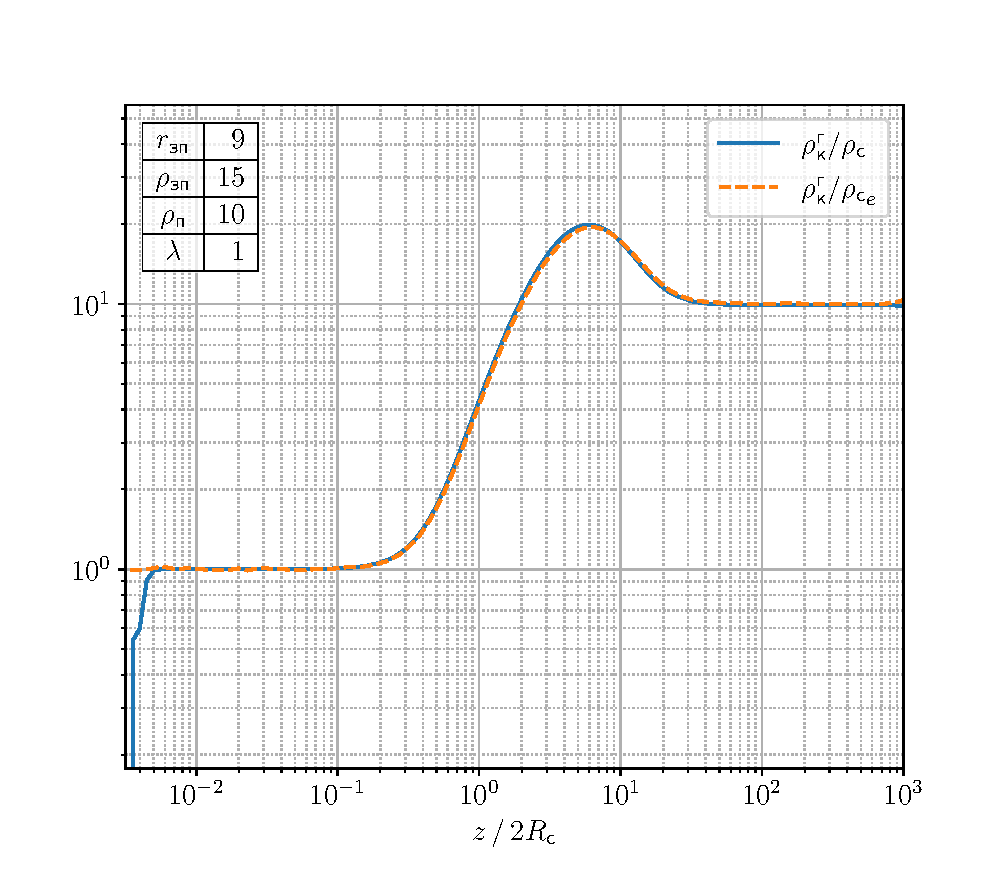
\includegraphics{exps/last_curves}
\caption{Кажущееся сопротивление}
%\label{fig:plot}
\end{figure}

\begin{figure}[H]
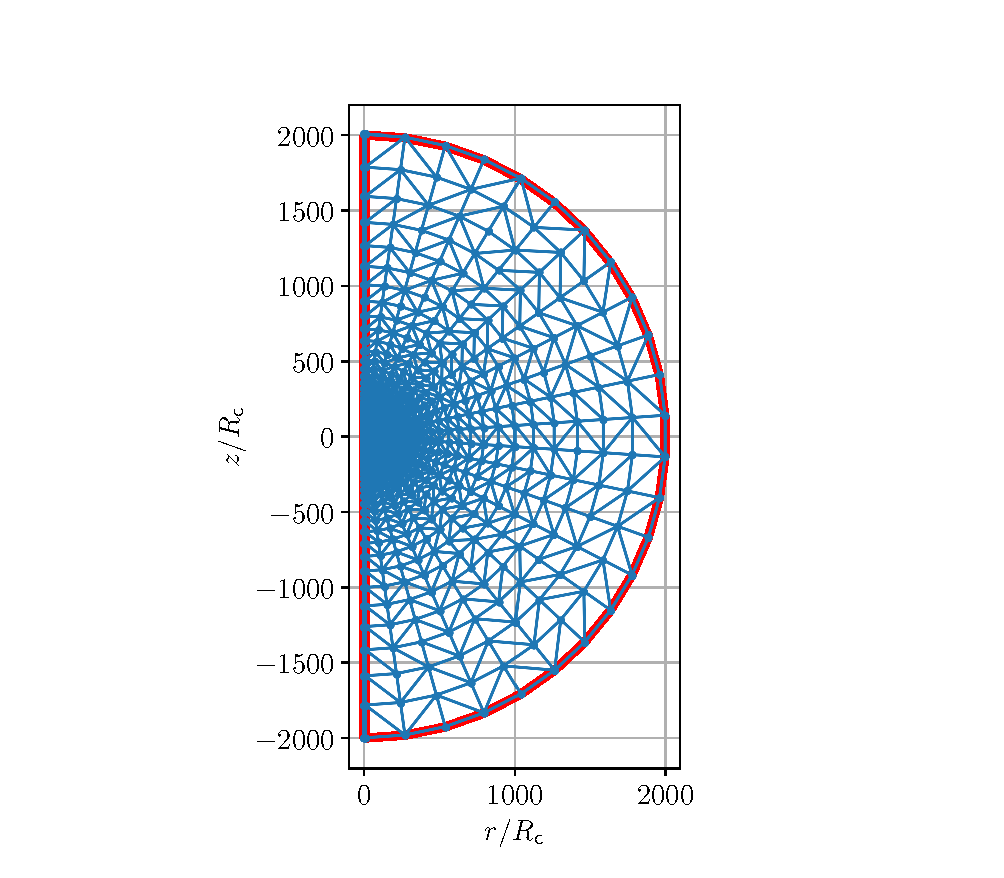
\includegraphics{exps/last_tg_1}
\caption{Триангуляция}
%\label{fig:plot}
\end{figure}

\begin{figure}[H]
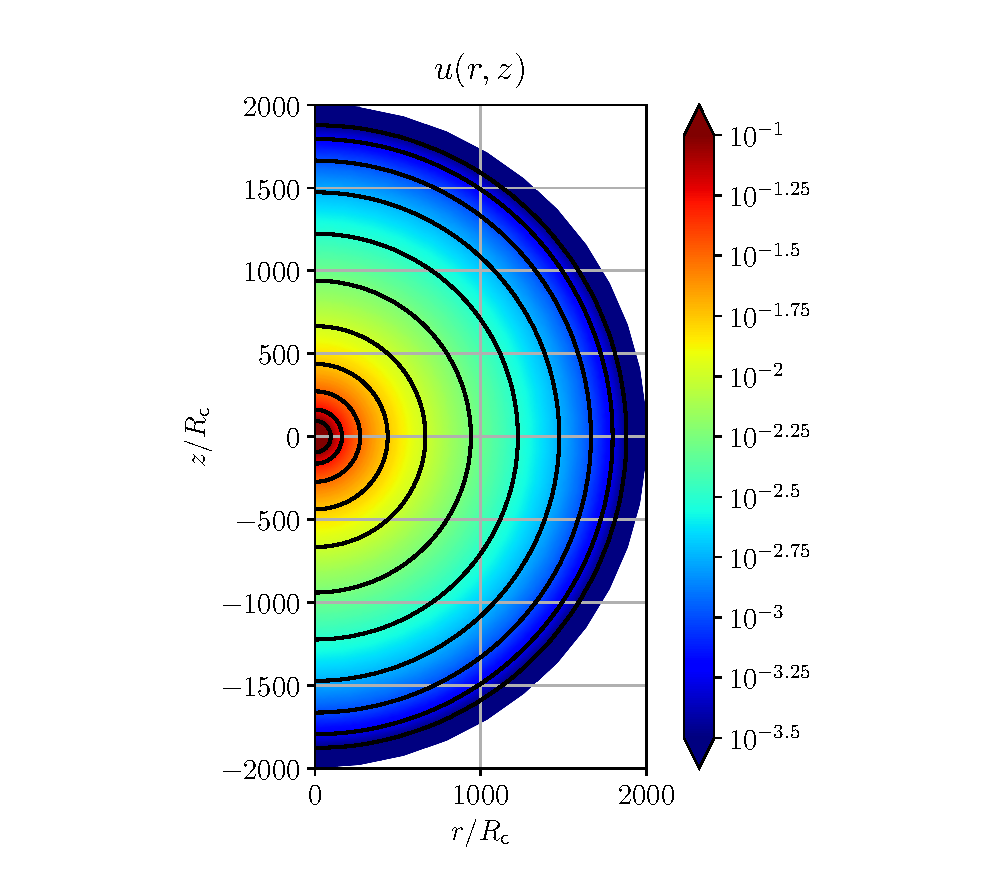
\includegraphics{exps/last_field_1}
\caption{Решение потенциального поля}
%\label{fig:plot}
\end{figure}

\begin{figure}[H]
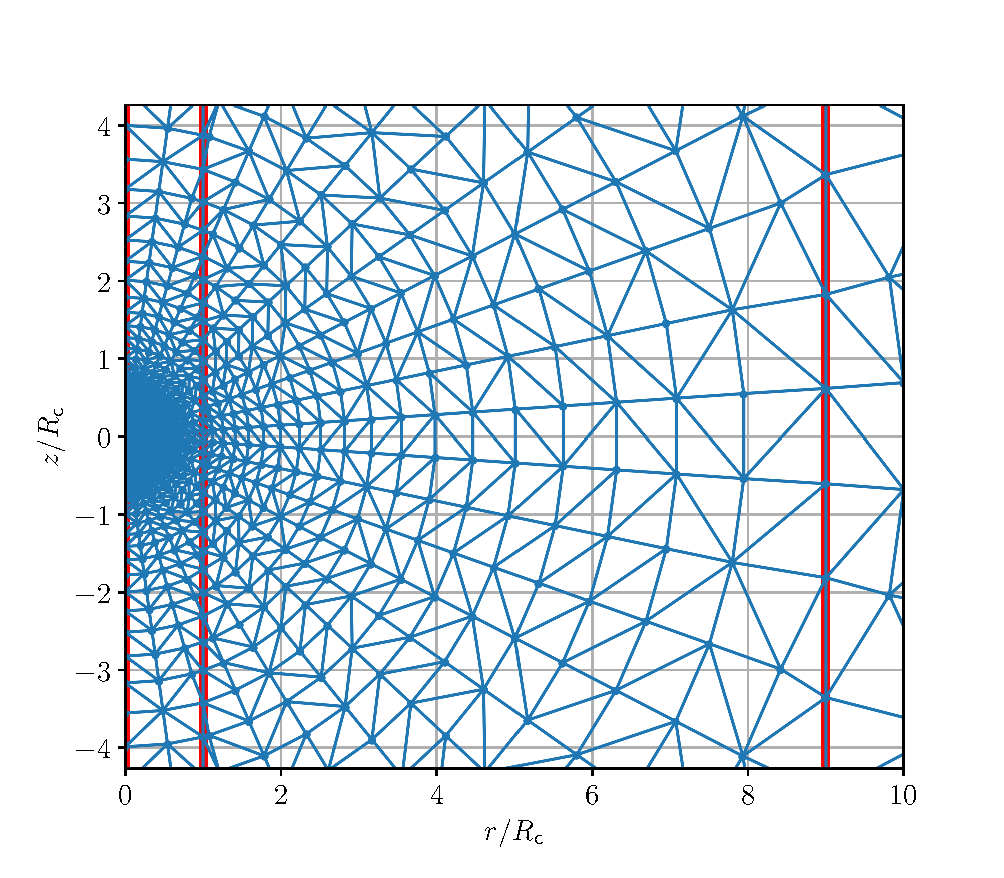
\includegraphics{exps/last_tg_2}
\caption{Триангуляция}
%\label{fig:plot}
\end{figure}

\begin{figure}[H]
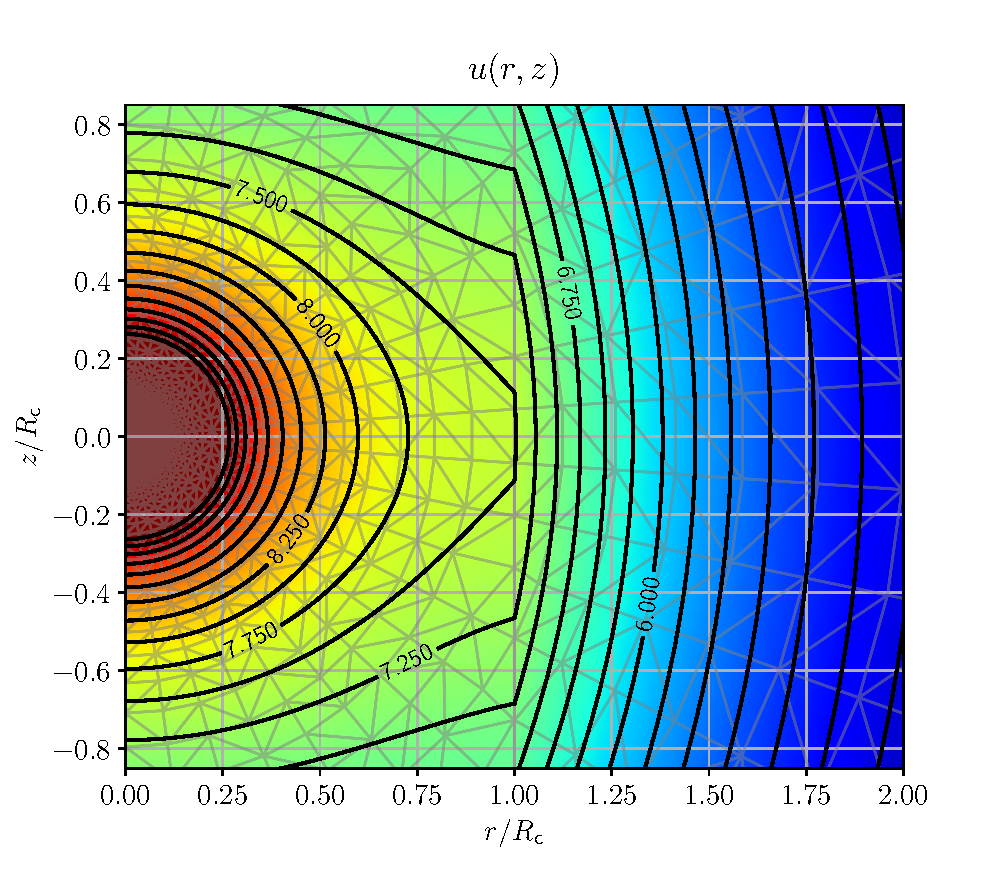
\includegraphics{exps/last_field_2}
\caption{Решение потенциального поля}
%\label{fig:plot}
\end{figure}


\subsection{Результаты}

Лучший результат получен в эксперименте \ref{best} за ${538 \text{ мc } \pm 37.8 \text{ мс }}$, 7 проходов
(${\text{среднее значение} \pm \text{среднеквадратичное отклонение}}$ от 7 проходов, в каждом проходе 1 цикл). Использованы узлы, равноотстоящие в логарифмическом масштабе; узлы лежащие в местах пересечений границ областей УЭС с концентрическими окружностями и лучами, отрезки графа на местах разрыва коэффициента УЭС; лагранжевые элементы ${\mathcal{P}_2}$; настройка 'p' библиотеки triangle. Использован компьютер для вычисления: операционная система Ubuntu 18.04 LTS, процессор Intel Pentium 4415U 2.30 ГГц с 4 логическими процессорами ($1 \text{ физический процессор} \times 2 \text{ ядра в физическом процессоре} \times 2 \text{ потока в каждом ядре}$)..

В результате проведённых численных экспериментов разработан метод построения оптимальных сеток для решения задачи БКЗ на сетке, позволяющий получить приемлимое численное решение с меньшими затратами ресурсов. В данном случае мы следили за двумя параметрами: гладкостью решения и сравнением "на глаз" с известной палеткой. Поскольку принятая методика решения обратной задачи БКЗ основано на использованием палеток на "сравнении на глаз", то такой критерий годится. Относительная ошибка примерно ${<10}$ \%.

\clearpage %
\section{Решение}

\subsection{Модель 1}

Трёхслойная осесимметричная модель:

{\setlength\tabcolsep{2pt}
\begin{tabular}{rcl}
    первый слой &---& скважина (${0 < r < 1}$) с УЭС ${\rho_\text с = 1}$, \\
    второй слой &---& зона проникновения (${1 < r < r_\text{зп} = 4}$) с УЭС ${\rho_\text{зп} = 4}$, \\
    третий слой &---& пласт (${r > r_\text{зп}}$) с УЭС $\rho_\text{п}$.
\end{tabular}}

\begin{figure}[H]
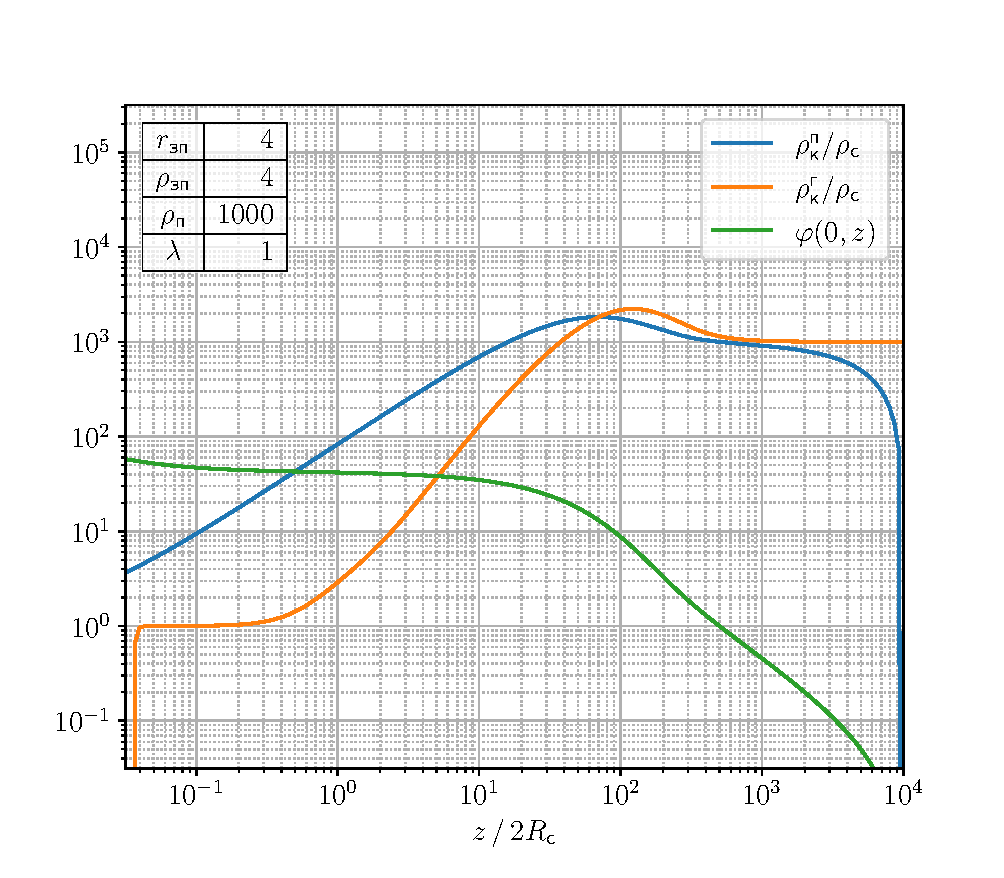
\includegraphics{plot_1_curves}
\caption{}
\label{fig:plot_1_curves}
\end{figure}

Время вычисления решения (рис. \ref{fig:plot_1_curves}) ${1.24 \text{ c } \pm 38.3 \text{ мс}}$, 7 проходов
(${\text{среднее значение} \pm \text{среднеквадратичное отклонение}}$ от 7 проходов, в каждом проходе 1 цикл).

6409 узлов расчетной сетки.

Далее изображены поле, расчетная сетка и решение для палетки с этой расчетной сеткой.

\begin{figure}[H]
\centering
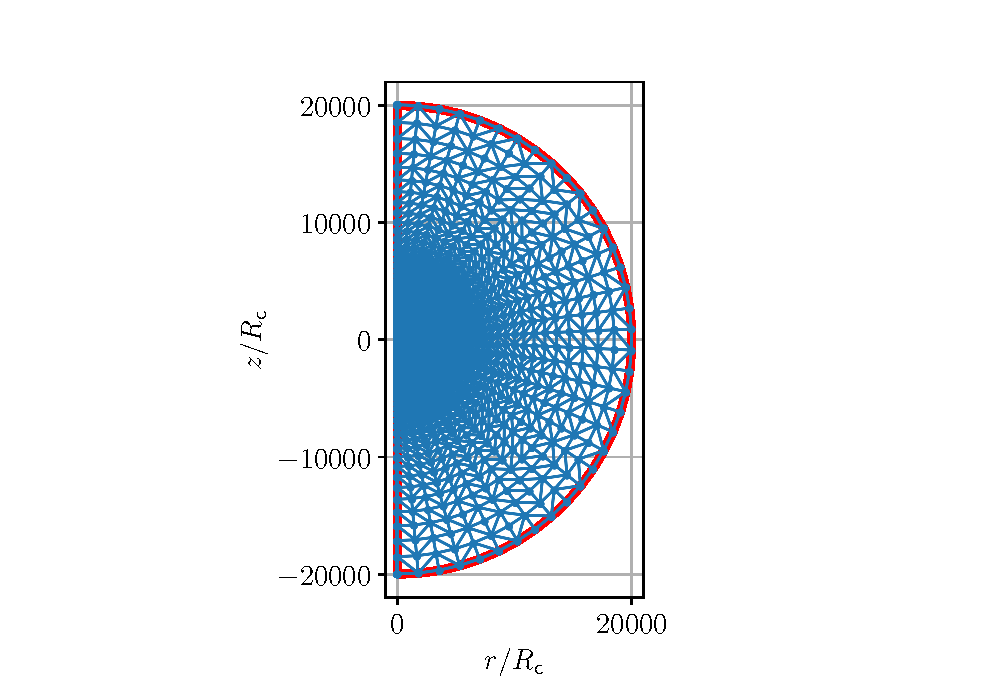
\includegraphics{plot_1_tg_1}
\caption{}
%\label{fig:plot}
\end{figure}

\begin{figure}[H]
\centering
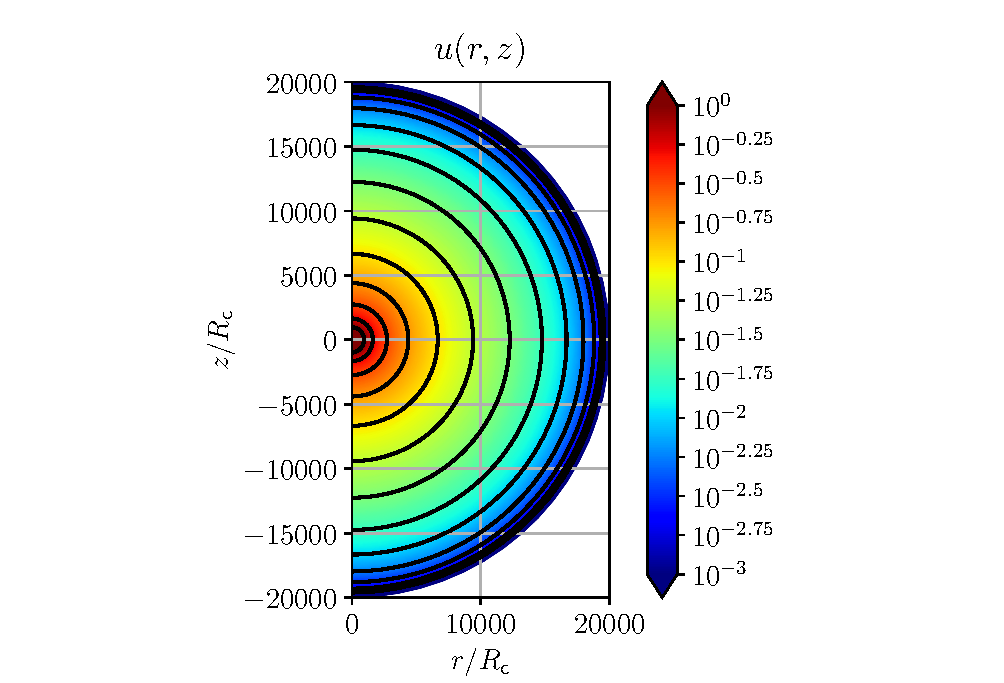
\includegraphics{plot_1_field_1}
\caption{}
%\label{fig:plot}
\end{figure}

\begin{figure}[H]
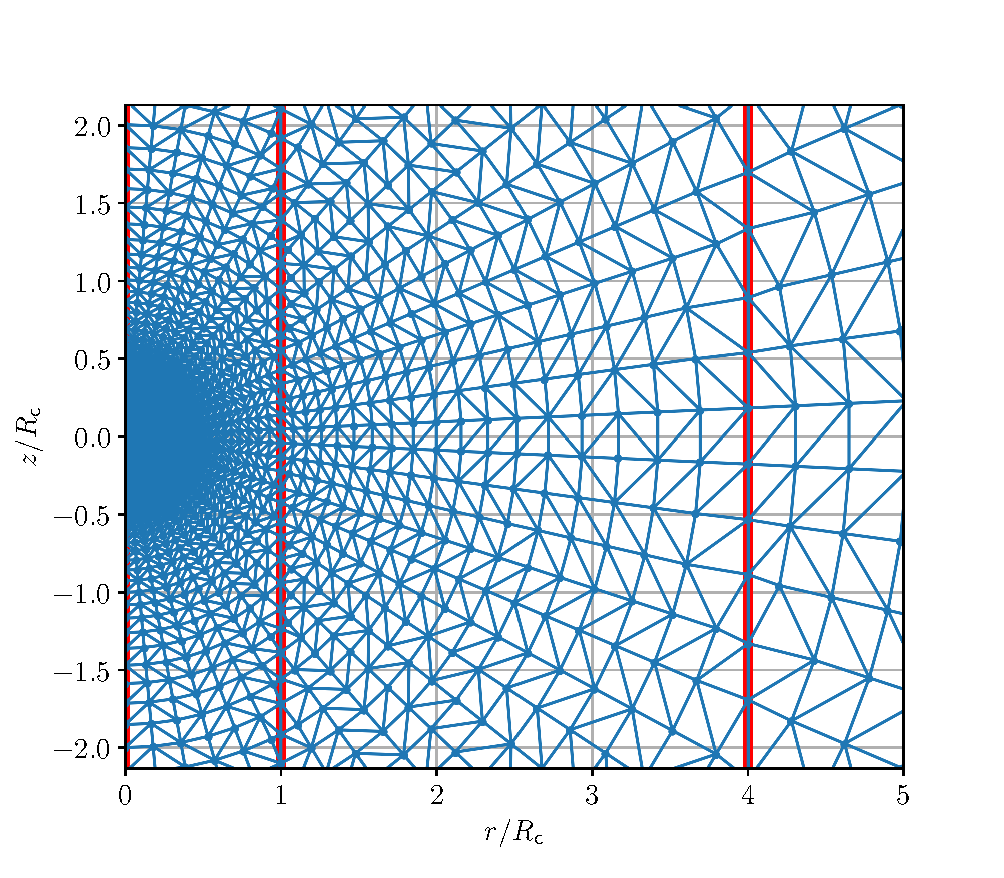
\includegraphics{plot_1_tg_2}
\caption{}
%\label{fig:plot}
\end{figure}

\begin{figure}[H]
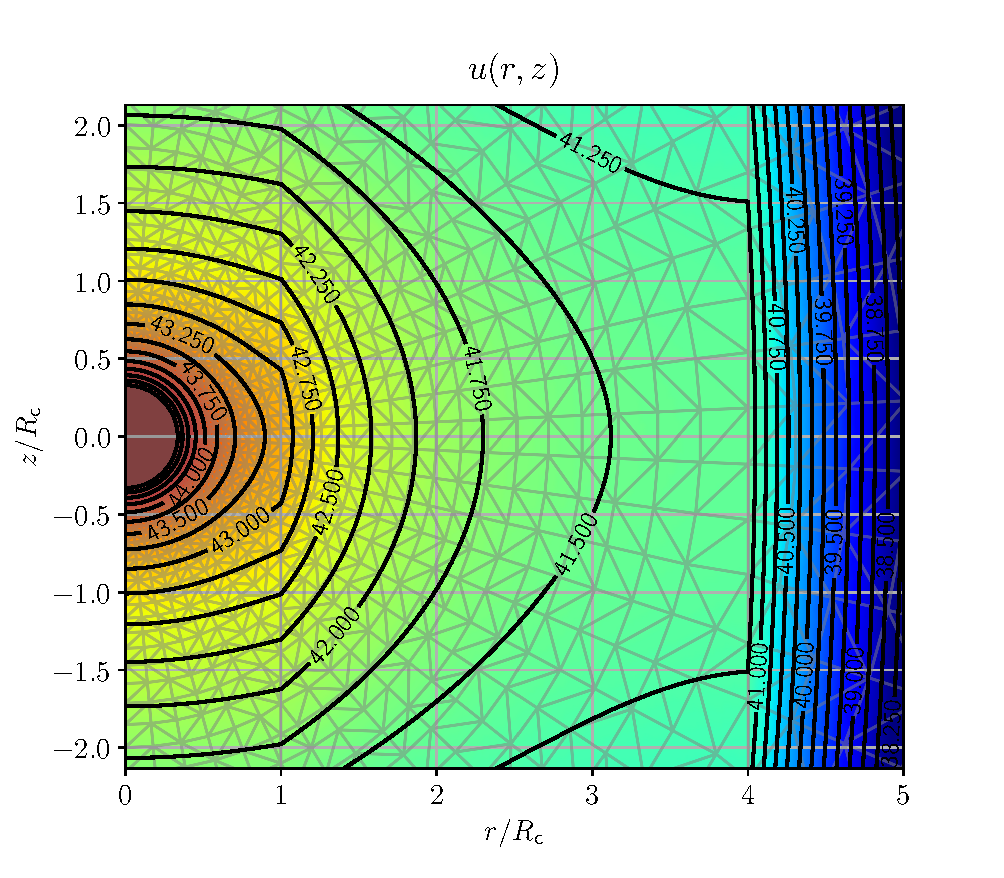
\includegraphics{plot_1_field_2}
\caption{}
%\label{fig:plot}
\end{figure}

\begin{figure}[H]
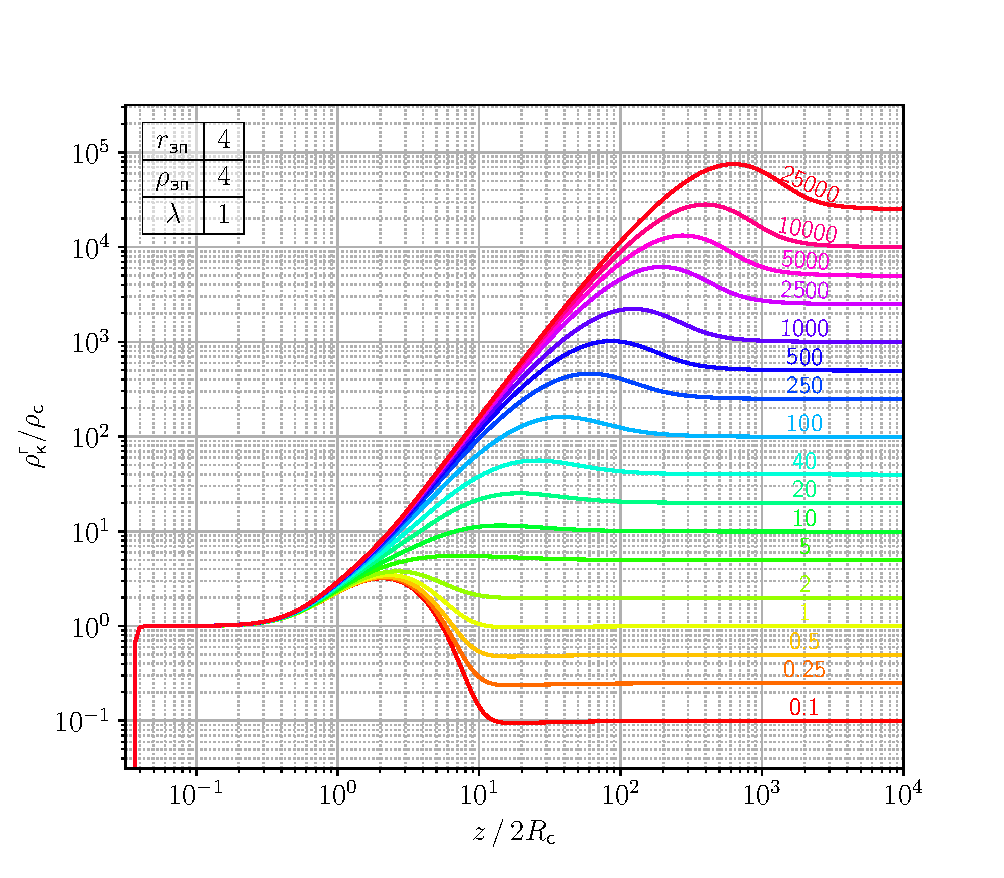
\includegraphics{plot_1_palette}
\caption{}
\end{figure}

Время вычисления палетки ${18 \text{ c } \pm 159 \text{ мс}}$, 7 проходов.


\begin{figure}[H]
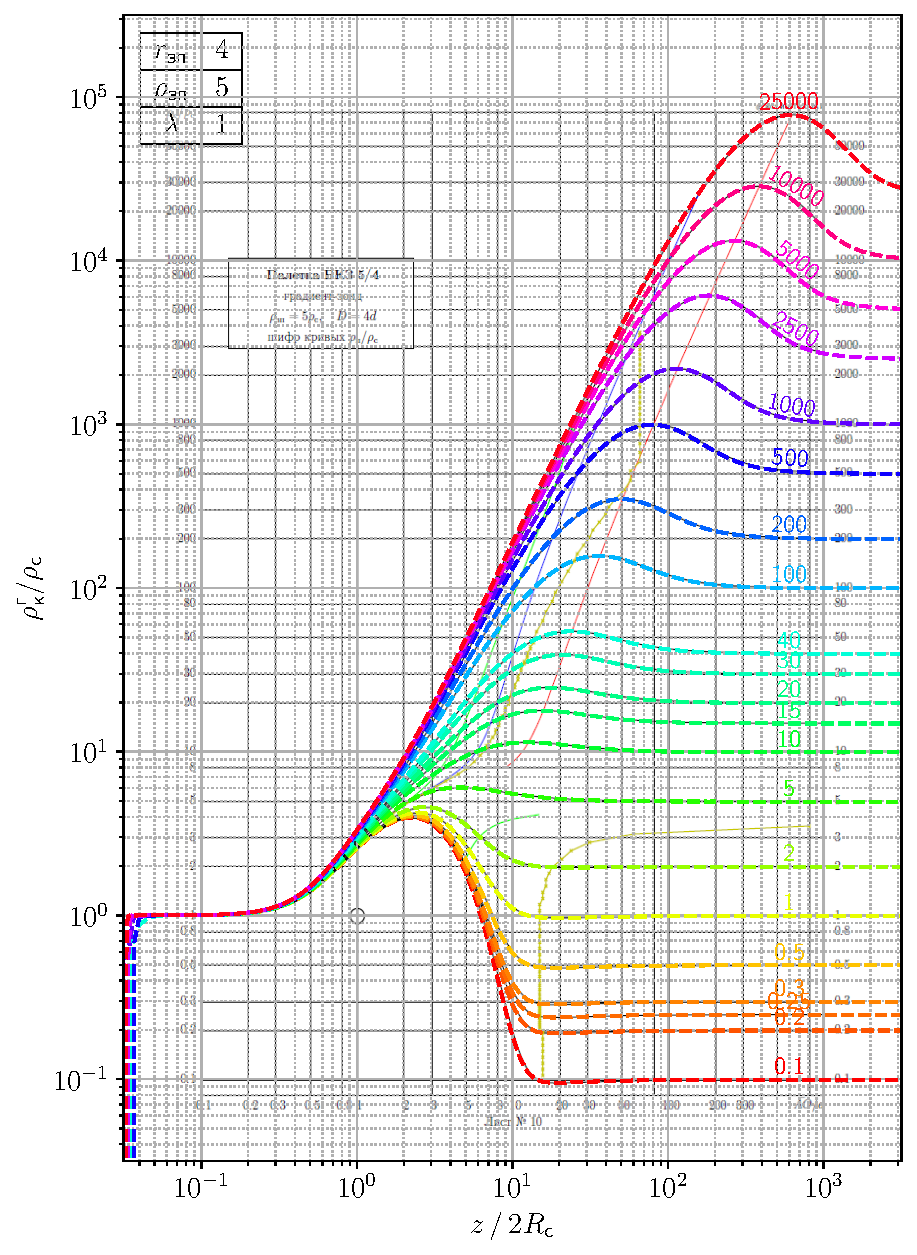
\includegraphics{plot_1_compare}
\caption{}
\end{figure}


\newpage
\subsection{Модель 2}

Четырехслойная осесимметричная модель с анизотропией:

\noindent
{\setlength\tabcolsep{2pt} \setlength\intextsep{0mm}
\begin{tabularx}{\linewidth}{r c X}
    первый слой &---& скважина (${0 < r < 1}$)
        с УЭС ${\rho_\text с = 1}$
        с коэффициентом анизотропии ${\lambda_\text{с} = 1}$, \\
    второй слой &---& промытая зона (${1 < r < r_\text{пз} = 2.2}$)
        с УЭС ${\rho_\text{пз} = 4}$
        с коэффициентом анизотропии $\lambda_\text{пз} = \lambda = 1.1$, \\
    третий слой &---& зона проникновения (${r_\text{пз} < r < r_\text{зп} = 5.8}$)
        с УЭС линейная функция от $r$ со значениями ${\rho_\text{зп}(r_\text{пз}) = \rho_\text{пз}}$
        и ${\rho_\text{зп}(r_\text{зп}) = \rho_\text{п}}$
        с коэффициентом анизотропии $\lambda_\text{пз} = \lambda = 1.1$, \\
    четвертый слой &---& пласт (${r > r_\text{зп}}$)
        с УЭС $\rho_\text{п}$
        с коэффициентом анизотропии $\lambda_\text{п} = \lambda = 1.1$.
\end{tabularx}}

\begin{figure}[H]
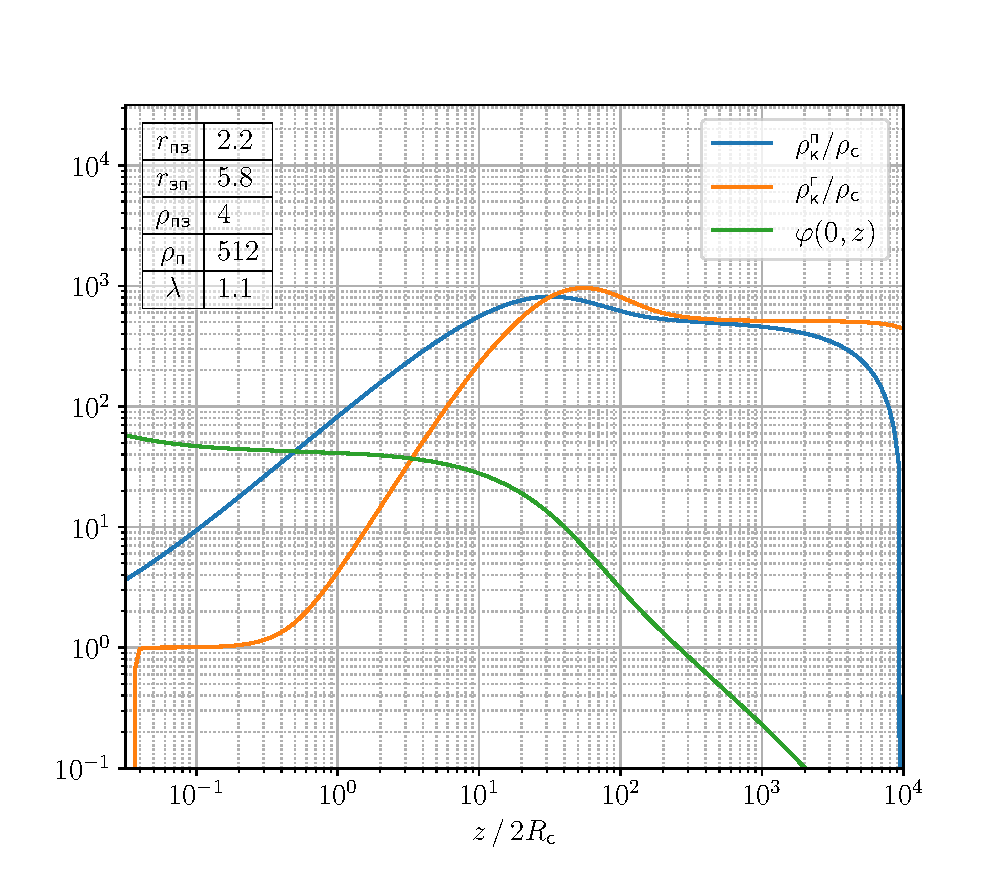
\includegraphics{plot_2_curves}
\caption{}
%\label{fig:plot}
\end{figure}

Время вычисления решения ${1.23 \text{ c } \pm 16.3 \text{ мс}}$, 7 проходов.

6613 узлов расчетной сетки.

Далее изображены поле, расчетная сетка и решение для палетки с этой расчетной сеткой.

\begin{figure}[H]
\centering
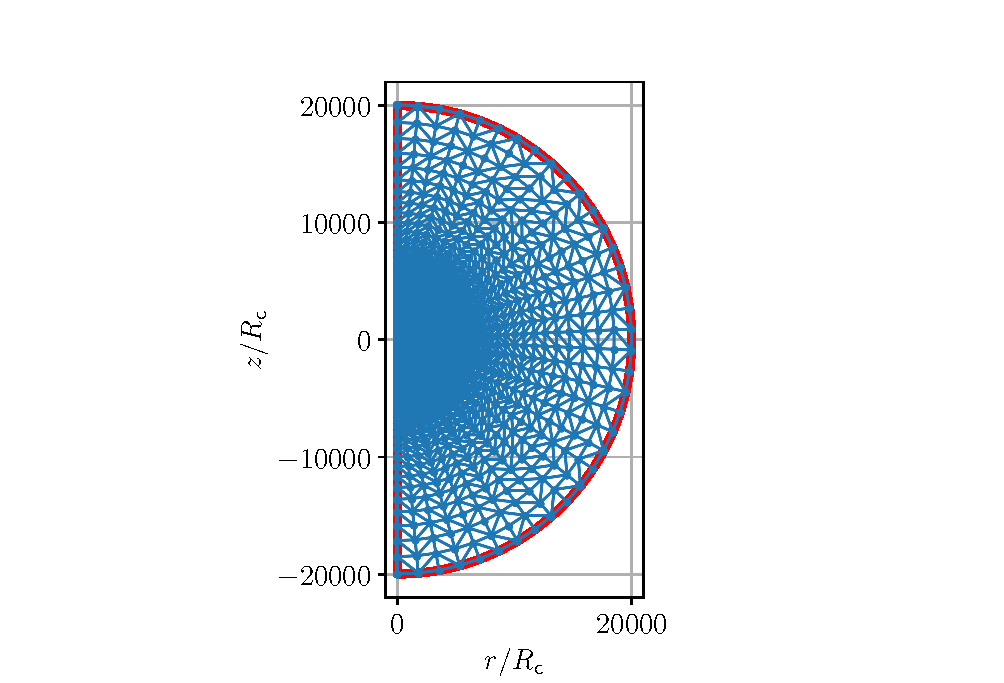
\includegraphics{plot_2_tg_1}
\caption{}
%\label{fig:plot}
\end{figure}

\begin{figure}[H]
\centering
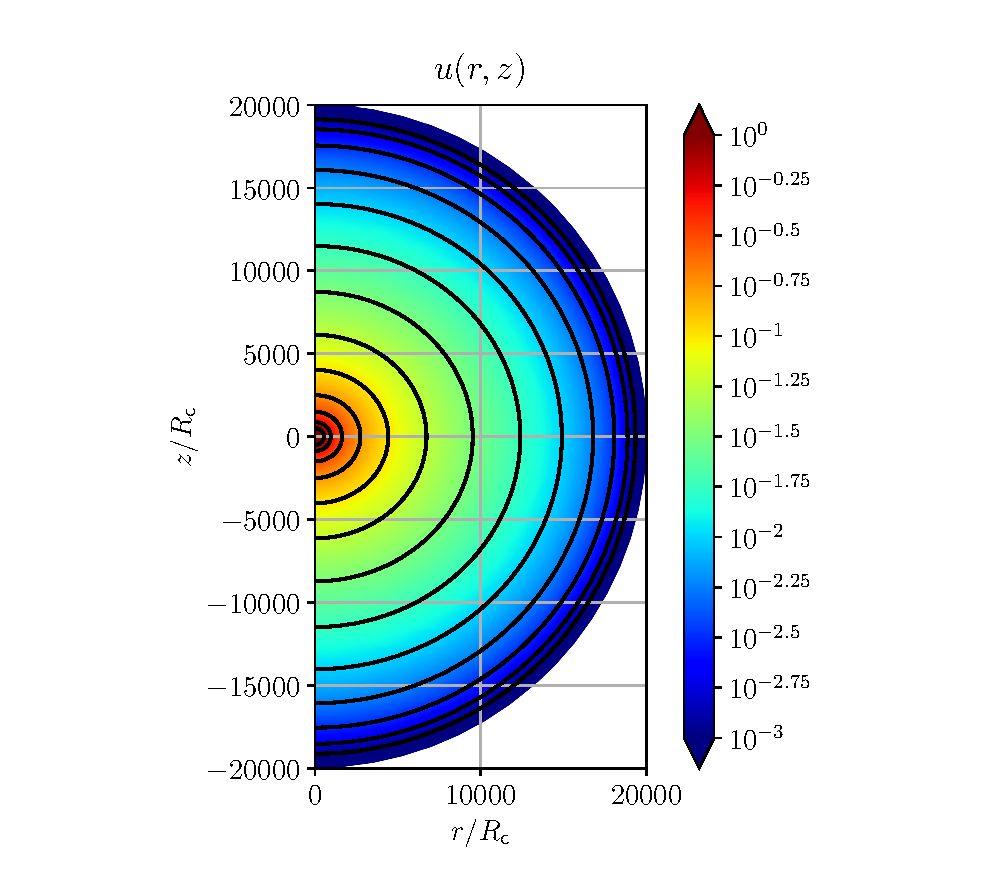
\includegraphics{plot_2_field_1}
\caption{}
%\label{fig:plot}
\end{figure}

\begin{figure}[H]
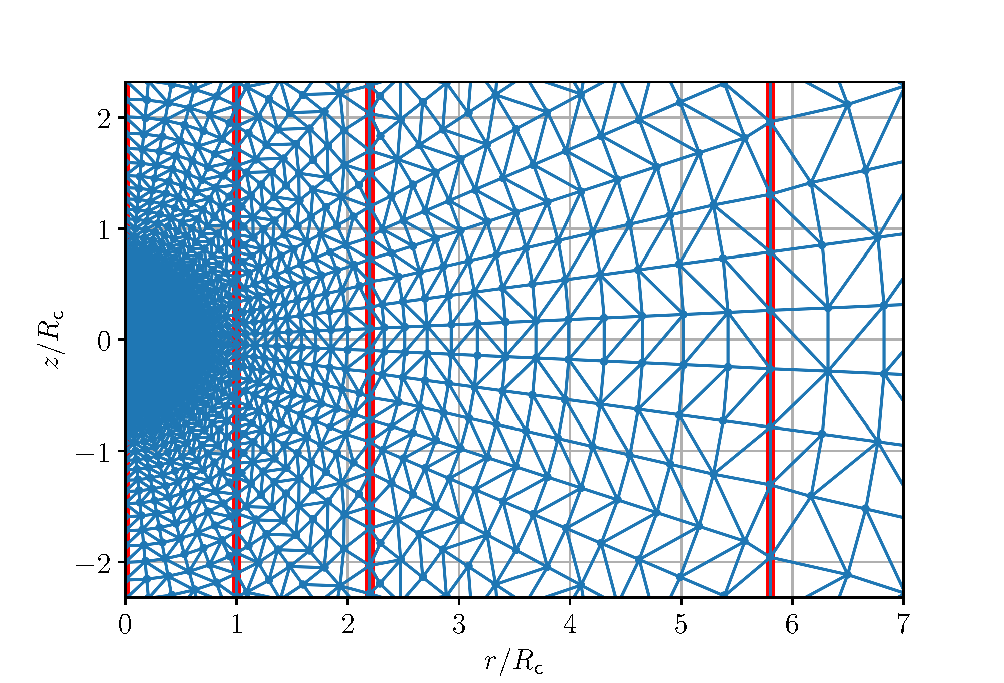
\includegraphics{plot_2_tg_2}
\caption{}
%\label{fig:plot}
\end{figure}

\begin{figure}[H]
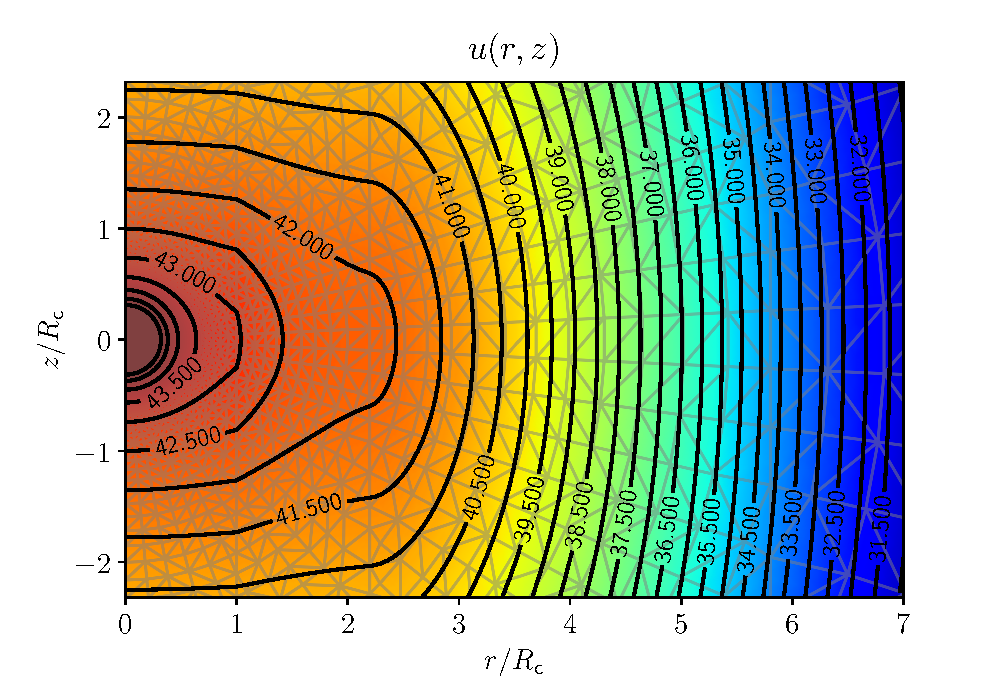
\includegraphics{plot_2_field_2}
\caption{}
%\label{fig:plot}
\end{figure}

\begin{figure}[H]
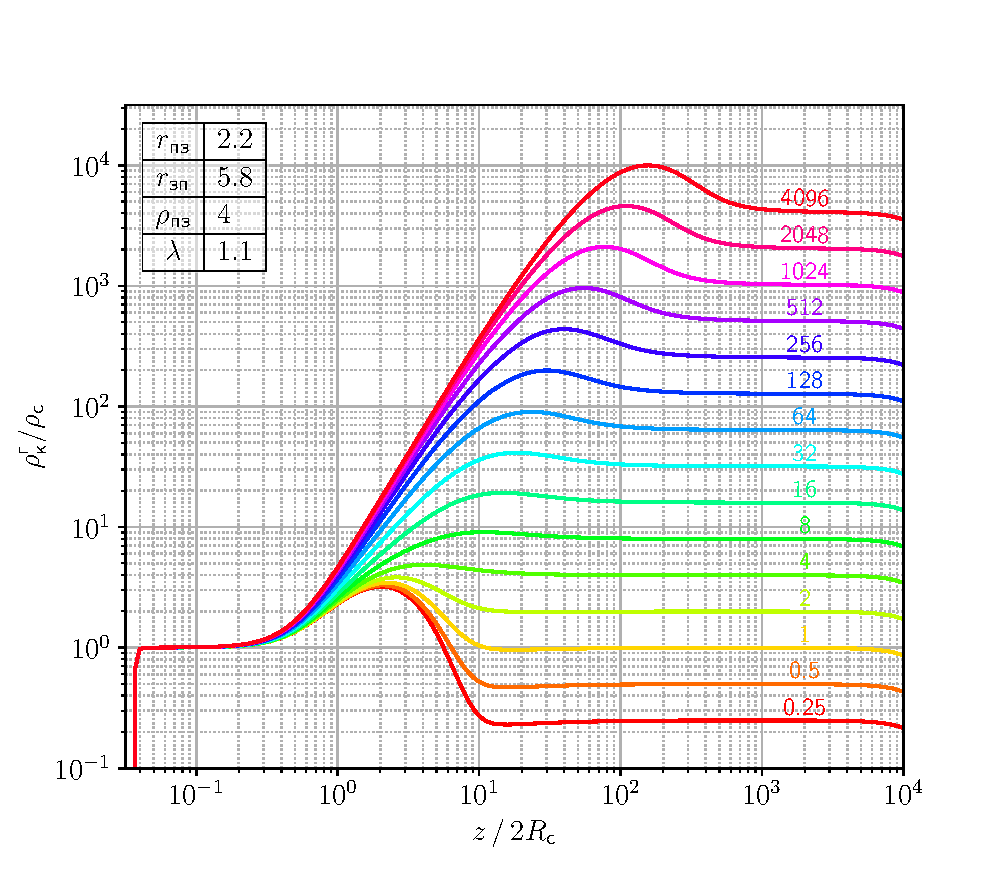
\includegraphics{plot_2_palette}
\caption{}
\end{figure}

Время вычисления палетки ${16.5 \text{ c } \pm 176 \text{ мс}}$, 7 проходов.

\begin{figure}[H]
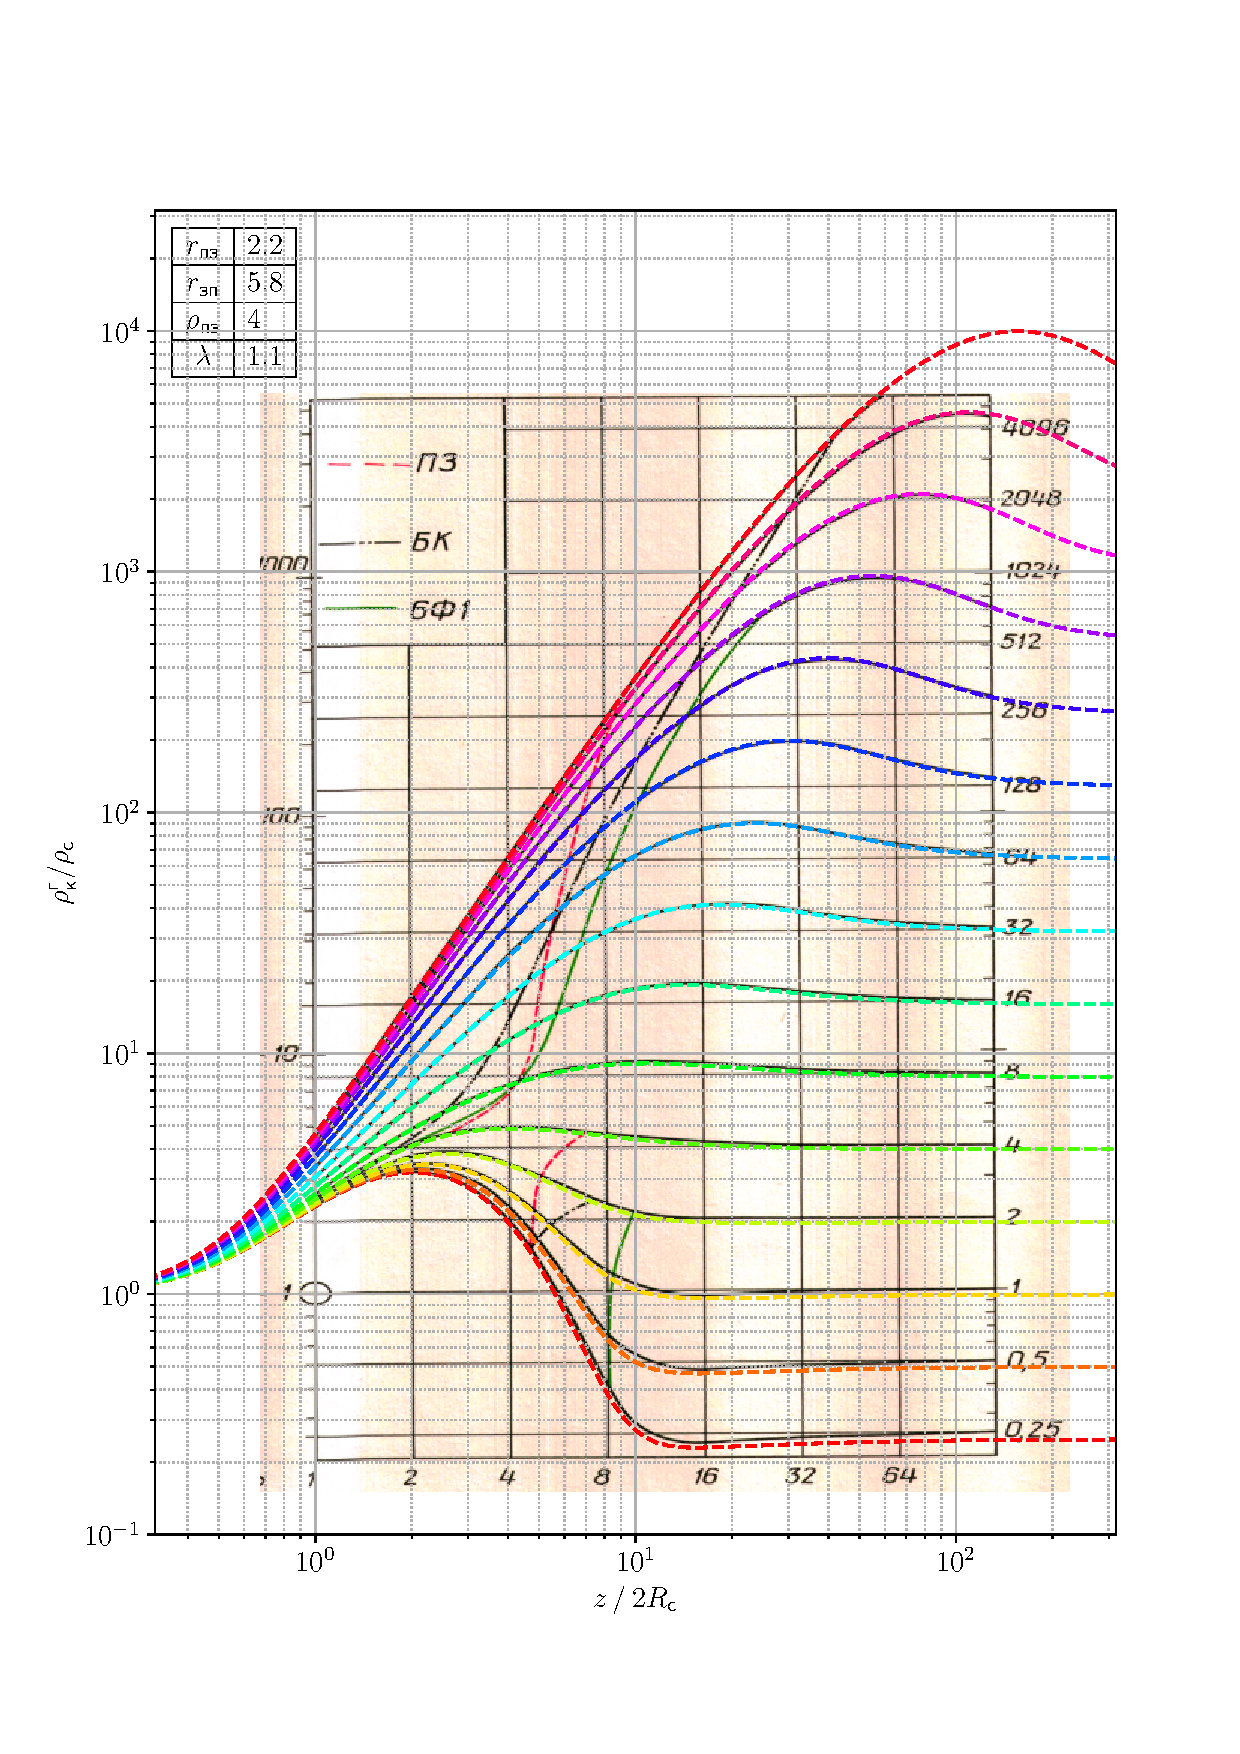
\includegraphics{plot_2_compare}
\caption{}
\end{figure}

\clearpage
 %
\anonsection{Заключение}

Показана применимость метода решения прямой задачи БКЗ с приемлимой точностью.

Текущая реализация метода является прототипом, требуется оптимизация реализации.

Необходимо исследование погрешности метода для курса дальнейшей работы.



\clearpage
 % Заключение
\begingroup 
\renewcommand{\section}[2]{\anonsection{Библиографический список}}
\begin{thebibliography}{00}

\bibitem{elec}
    Электрическое зондирование геологической среды. Часть 1. Прямые задачи и методика работ /
    И. Н. Модин, В. А. Шевнин, В. К. Хмелевской [и др.]
    --- МГУ Москва, 1988.
    --- 176 с.
    --- URL: \url{http://geophys.geol.msu.ru/STUDY/5KURS/Book1_1988MSU.pdf}

\bibitem{FEM_intro}
    Введение в теорию метода конечных элементов. Учебное пособие /
    Р.З. Даутов, М.М. Карчевский.
    --- Казань: Казанский государственный универcитет им. В.И. Ульянова–Ленина, 2004.
    --- 239 с.
    --- URL: \url{https://kpfu.ru/staff_files/F1229619272/MKEbookDRZ.pdf}

\bibitem{palette}
    Технология создания многопараметричных
    палеток для решения прямых и обратных задач
    скважинной геоэлектрики /
    К. С. Сердюк [и др.]
    Каротажник. Результаты исследований и работ ученых и конструкторов, 2014.
    --- Вып. 241.
    --- С. 32-41.

\bibitem{valiullin}
    Геофизические исследования и работы в скважинах: в 7 т. Т. 1.
    Промысловая геофизика /
    Р.А. Валиуллин, Л.Е. Кнеллер.
    --- Уфа: Информреклама, 2010.
    --- 172 с.


\bibitem{none}
    Методические указания по комплексной интерпретации данных БКЗ, БК, ИК (с комплектом палеток) /
    Науч.-произв. об-ние "Союзпромгеофизика", Всесоюз. н.-и. и проект.-конструкт. ин-т геофиз. методов исслед., испытания и контроля нефтегазоразведоч. скважин. Е. В. Чаадаев, И. П. Бриченко, А. А. Левченко [и др.]
    --- Калинин: НПО "Союзпромгеофизика", 1990.
    --- 85 с.
   
\bibitem{FEFIS}
    Finite Elements and Fast Iterative Solvers: with Applications in Incompressible Fluid Dynamics (2nd edition) /
    H. Elman, D. Silvester, A. Wathen.
    --- OUP, Oxford, 2014. 
    --- 480 с.
    --- URL: \url{https://books.google.ru/books?id=Ly-TAwAAQBAJ}

\bibitem{FEniCS}
    Solving PDEs in Python --The FEniCS Tutorial Volume I /
    H. P. Langtangen, A. Logg.
    --- Springer, 2017.
    --- 153 с.
    --- URL: \url{https://fenicsproject.org/pub/tutorial/pdf/fenics-tutorial-vol1.pdf}

\end{thebibliography}
\endgroup

\clearpage
 % Библиографический список
\vspace*{\fill}
\centering{\uppercase{Приложение}}
\vspace*{\fill}

\clearpage

\appsection{Приложение А}
\centering{\uppercase{Вариант программы на Python для расчета сеток}}
\vspace{\baselineskip}

\lstinputlisting[numbers=left]{inc/scripts/mesh.py}
% \inputminted{python}{inc/scripts/mesh.py}

\clearpage
 % Вариант программы на Python для расчета сеток

\end{document}
%%% Конец документа
